\section{Quark and Hadron Universe}\label{part2}
%%%%%%%%%%%%%%%%%%%%%%%%%%%%%%%%%%%%%%%%%
\subsection{Heavy particles in QGP epoch}
\label{HiggsQGP}
%%%%%%%%%%%%%%%%%%%%%%%%%%%%%%%%%%%%
\para{Matter phases in extreme conditions}
This section will be focused on a few examples of interest to cosmological context. In the temperature domain below electroweak boundary near $T=130$\,GeV we explore in preliminary fashion novel and interesting physical processes. We will consider the Higgs\index{Higgs}, meson, and the heavy quarks $t,b,c$ with emphasis on bottom quarks\index{bottom quark}. We will show that the bottom quarks can deviate from chemical equilibrium\index{chemical equilibrium} $\Upsilon\neq 1$ by breaking the detailed balance between production and decay reactions. It is easy to see considering temperature scaling and additional degrees of freedom that the energy density of matter near to electroweak phase transition is a stunning 12 orders of magnitude greater compared to the benchmark we discussed for QGP-hadronization\index{hadrons!hadronization}, see~\req{endensval}.
 
The dynamical bottom $ b,\bar b$-quark pair abundance depends on the competition between the strong interaction two gluon fusion process into $b\bar b$-pair and weak interaction decay rate of these heavy quarks. This lead to the off-equilibrium phenomenon of the bottom quark freeze-out in abundance near the hadronization temperature as discussed in Ref.\,\cite{Yang:2020nne} and below. Here we further argue that the same unusual situation could exist for any other heavy particle in QGP at a temperature well below their mass scale. We study as an example the abundance of the Higgs particle at condition $m_H\gg T$. Higgs is a particularly interesting case due to its special position in the particle ZOO and a narrow width.

We also explore the properties of hadronic phase after hadronization with special emphasis on gaining an understanding about the strangeness $s,\bar s$ content of the Universe which persists to unexpectedly low temperature. Many of the methods we use in this context were developed in order to understand the properties of strongly interacting QGP formed in relativistic \ie\ high-energy heavy-ion\index{heavy-ion!collisions} \ie\ nuclear collision experiments. Such experimental program is in progress at the Relativistic heavy-ion Collider (RHIC) at BNL-New York\index{BNL!RHIC} and the Large Hadron Collider (LHC) at CERN\index{CERN!LHC}. 

Let us remind the reasons why the dynamics of particles and plasma in the primordial Universe differs greatly from the laboratory environment. We focus here on the case of QGP-hadron phase boundary but a similar tabular list applies to other era boundaries:\index{Big-Bang!difference with laboratory}
\begin{enumerate} 
\item The primordial Big-Bang QGP epoch lasts for about $20\,\mu$s. On the other hand, the QGP formed in collision micro-bangs has a lifespan of around $10^{-23}$\,s. 
\item In the primordial Universe the microscopic transformation of quarks into hadrons proceeded through creation of the so called mixed phase allowing for local equilibration and a full relaxation of strongly interacting degrees of freedom during about $10\,\mu$s~\cite{Fromerth:2002wb}. Current lattice QCD models predict a smooth transformation. The transformation in the laboratory is much closer to what can be called explosive and sudden conversion of quarks into hadronic (confined) degrees of freedom~\cite{Rafelski:2000by}. Such a situation can mimic phenomena usually observed in a true phase transition of first order.
\item Half of the degrees of freedom present in the Universe (charged leptons, photons, neutrinos) are not part of the thermal laboratory micro-bang.
\item Experimental reach today is at and below $T\simeq 0.5$\,GeV allowing to explore the hadronization process of the QGP but not the heavy particle (H,W,Z,$t$) content, $b$ and $c$ quarks are difficult to study. 
\item Though the baryon content of the laboratory QGP is very low it is probably also much higher compared to the observed baryon asymmetry\index{baryon!asymmetry} in the Universe. 
\end{enumerate}
 
%%%%%%%%%%%%%%%%%%%%%%%%%%%%%%%%%%%
\para{Higgs equilibrium abundance in QGP} 
We would like to show that it is of interest to study the Higgs\index{Higgs} particle dynamics at relatively late stage of Universe evolution. This is an ongoing project which is described here for the first time. We are now considering in the primordial Universe the temperature range $10\,\mathrm{GeV}>T>1\,\mathrm{GeV}$, and recall the mass of the Higgs particle $m_H\simeq 125\GeV$. Therefore the number density of the Higgs can be written using the relativistic Boltzmann\index{Boltzmann!approximation} approximation
\begin{align}
n_{H}=\frac{\Upsilon_H}{2\pi^2}T^3\left(\frac{m_H}{T}\right)^2 K_2(m_H/T)\,.
\end{align}\index{Higgs!particle abundance}

We are interested to compare the abundance of the Higgs particle to the net abundance of baryon excess over antibaryons\index{baryon!antibaryon} to determine at which temperature the Higgs particle yield drops below this tiny Universe asymmetry. Our interest derives from the question how far down in temperature a baryon number breaking Higgs decay could be of relevance. Clearly, once the Higgs yield falls far below baryon asymmetry it would be difficult to argue it can contribute to grow the baryon asymmetry in the Universe. Moreover, comparing to baryon asymmetry seems to be a reliable measure of more general physical relevance, after all, our present Universe structure derives from this small asymmetry probably developed in the primordial epoch we explore here. 
 
The density between Higgs and baryon asymmetry (quark-antiquark asymmetry) can be written as
\begin{align}
\frac{n_H}{(n_B-n_{\bar{B}})}=\frac{n_{H}}{s_{tot}}\,\left(\frac{s_{tot}}{n_B-n_{\bar{B}}}\right)=
\frac{n_{H}}{s_{tot}}\left[\frac{s_{\gamma,\nu}}{n_B-n_{\bar{B}}}\right]_{t_0}\,.
\end{align}
Assuming no `late' baryon genesis and entropy conserving Universe expansion, we introduce in \req{BaryonEntropyRatio} in the last equality the present day value of baryon per entropy ratio\index{baryon!entropy ratio}. The entropy density\index{entropy!density} $s_{tot}$ in QGP can be obtained employing the entropic degrees of freedom $g^s_\ast$, \req{eq:entg} and~\rf{EntropyDOF:Fig}
\begin{align}
 &s_{tot}=\frac{2\pi^2}{45}g^s_\ast T_\gamma^3,\qquad g^s_\ast=\sum_{i=\mathrm{g},\gamma}g_i\left({\frac{T_i}{T_\gamma}}\right)^3+\frac{7}{8}\sum_{i=l^\pm,\nu,u,d}g_i\left({\frac{T_i}{T_\gamma}}\right)^3\,.
\end{align}
The entropy content to a good approximation is dominated by all effectively massless particles at given temperature in QGP. 

The baryon-to-photon density ratio $\eta$ today is bracketed by $5.8\times10^{-10} \leqslant\eta\leqslant6.5\times10^{-10}$ \cite{ParticleDataGroup:2018ovx}, a more precise value $\eta=(6.12\pm0.04)\times10^{-10}$~\cite{ParticleDataGroup:2022pth} is used in our study. This observed value is the evidence of baryon asymmetry and quantifies the matter-antimatter asymmetry in the Universe.\index{baryon!per photon ratio}

The density ratio between Higgs\index{Higgs} and baryon asymmetry for the case of chemical equilibrium $\Upsilon_H=1$ is seen in~\rf{HiggsDensity:fig}. At temperature $T=5.7\GeV$ this ratio is equal to unity. This implies that Higgs decay processes could populate and influence the baryon asymmetry down to this relatively low temperature scale. 

%%%%%%%%%%%%%%%%%%%%%%%%%%%%%%%%%%%%%%%%%%%%%%%%%%%%%%%%%%%%%%%%%%
\begin{figure}
\centerline{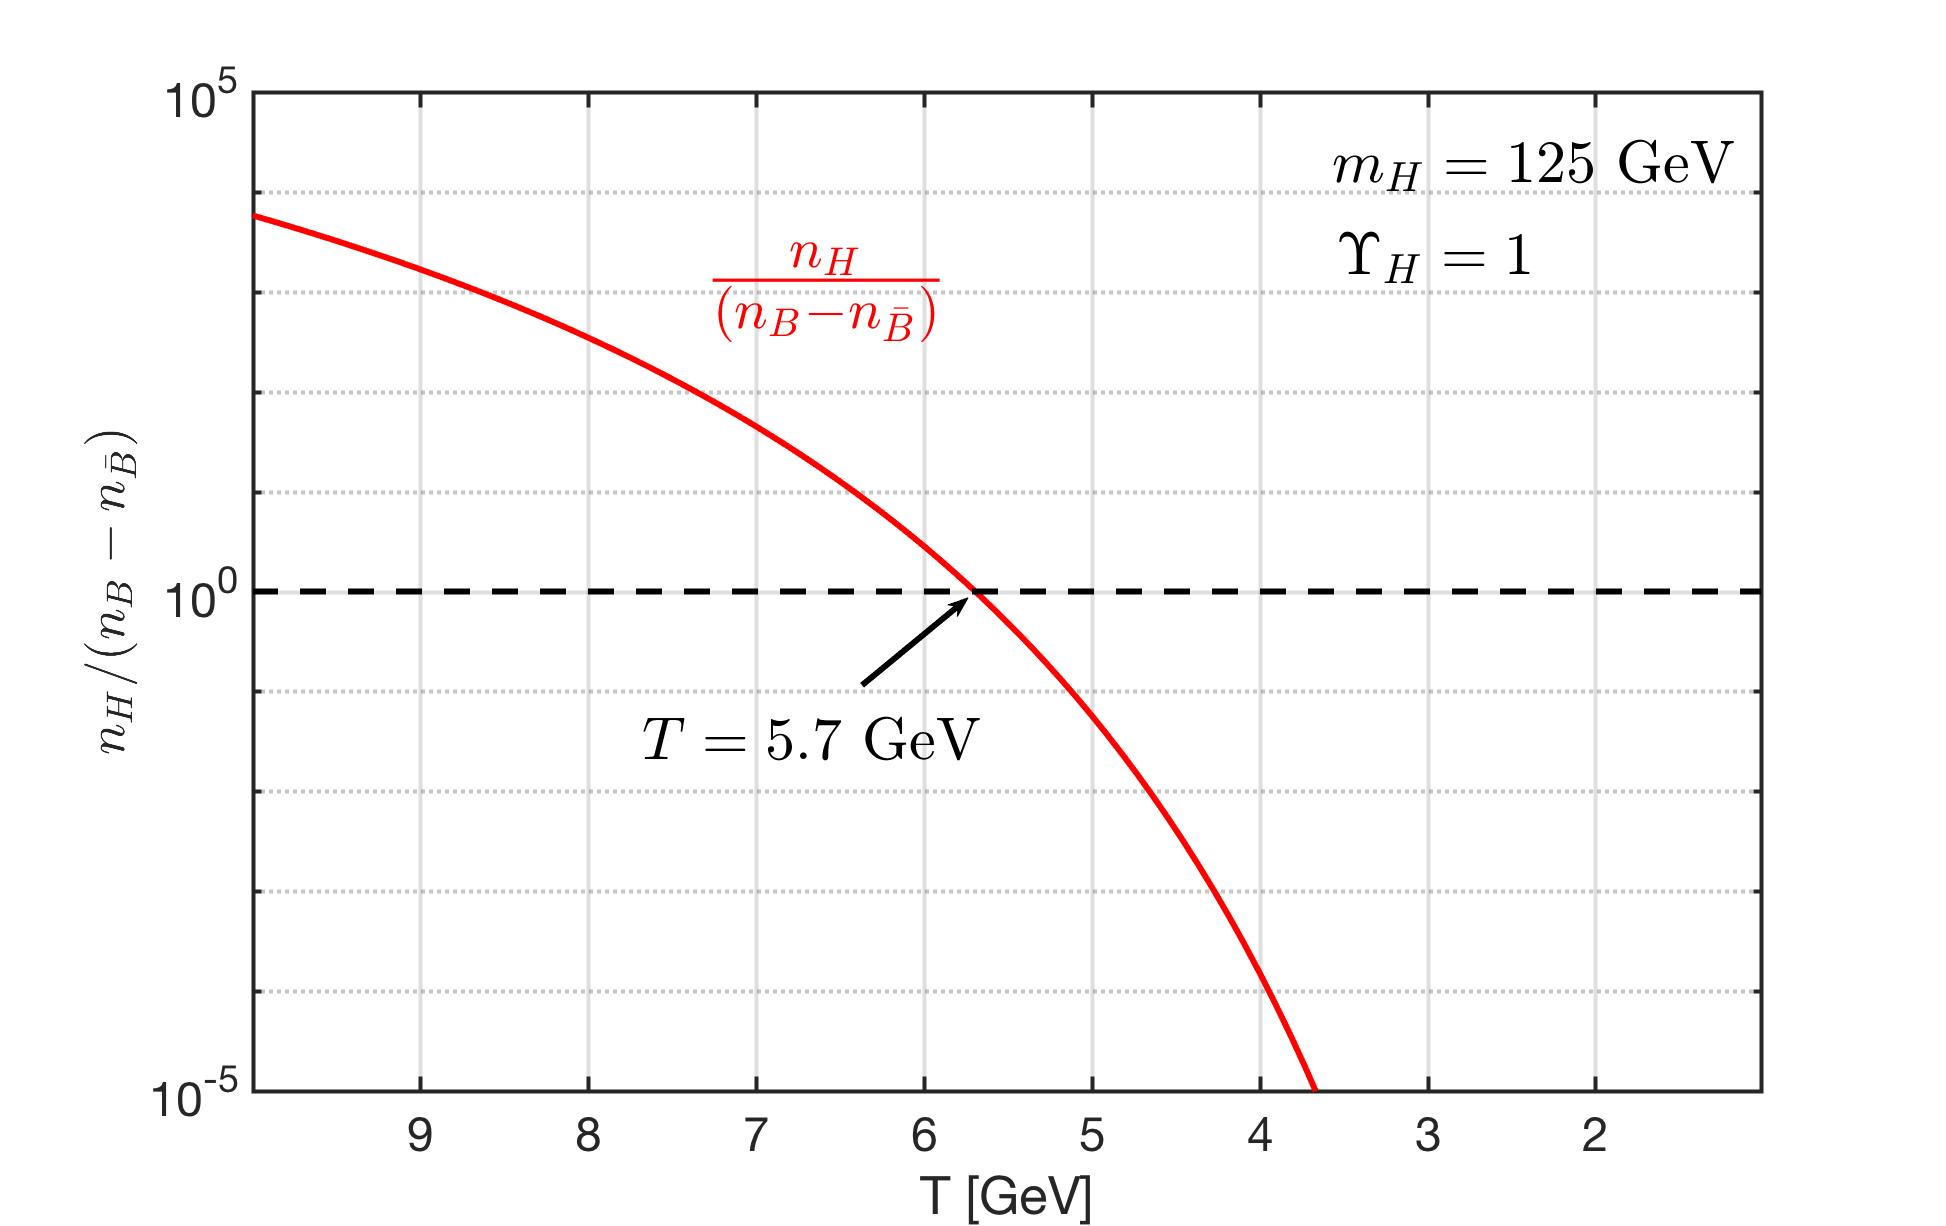
\includegraphics[width=0.9\linewidth]{./plots/HiggsDensityRatio}}
\caption{The ratio between Higgs density $n_H$ and baryon asymmetry density $n_B-n_{\bar B}$ as a function of temperature $T$ assuming chemical Higgs equilibrium $\Upsilon_H=1$ and present day entropy per baryon. Both densities are equal (horizontal line) at the temperature $T=5.7\GeV$. \radapt{Yang:2024ret}}
\label{HiggsDensity:fig} 
\end{figure}
%%%%%%%%%%%%%%%%%%%%%%%%%%%%%%%%%%%%%%%%%%%%%%%%%%%%%%%%%%%%%%%%%%%

%%%%%%%%%%%%%%%%%%%%%%%%%%%%
\para{Baryon asymmetry and Sakhraov conditions}\index{Sakharov conditions!baryogenesis}
The small value of the baryon asymmetry in the Universe could be interpreted as simply due to the initial conditions in the Universe. However, in the current standard cosmological model, it is believed that the inflation event can erase any pre-existing asymmetry between baryons and antibaryons. In this case, we need a dynamic baryogenesis process to generate excess of baryon number compared to antibaryon number in order to create the observed baryon number today.

The precise epoch responsible for the observed matter genesis $\eta$ in the primordial Universe has not been established yet. Several mechanisms have been proposed to explain baryogenesis with investigations typically focusing on the temperature range between GUT phase transition $T_\mathrm{G}\simeq10^{16}\,\mathrm{GeV}$ and the electroweak phase transition near $T_\mathrm{W}\simeq130\,\mathrm{GeV}$~\cite{Kuzmin:1985mm,Kuzmin:1987wn,Arnold:1987mh,Kolb:1996jt,Riotto:1999yt,Nielsen:2001fy,Giudice:2003jh,Davidson:2008bu,Morrissey:2012db}.

In following we present arguments that the Sakharov conditions~\cite{Sakharov:1967dj} for matter asymmetry to form also could appear during the QGP era: several heavy particles such as bottom quarks and including the Higgs as described above can fulfill nonequilibrium requirement. We will study below in more detail the bottom case and argue for the Higgs case. Other cases are possible.

In 1967, Andrei Sakharov formulated the three conditions necessary to permit baryogenesis in the primordial Universe~\cite{Sakharov:1967dj} and in 1991 he refined the three conditions as follows~\cite{Sakharov:1988vdp}:
\begin{itemize}
 \item Absence of baryonic charge conservation 
 \item Violation of CP-invariance\index{CP violation}
 \item Non-stationary conditions in absence of local thermodynamic equilibrium
\end{itemize}
 
In regard to first Sakharov condition: By assumption there is no initial asymmetry in baryon number in the Universe. Toady it is argued that an initial asymmetry could not survive the inflationary expansion. Furthermore ad-hoc Big-Bang baryon-antibaryon inherent asymmetry seems less attractive. In short we believe that the asymmetry between baryons and antibaryons we observe requires dynamic process and the presence of baryon number non-conserving reactions. 

The other option, an interaction which favors agglomerations of same `sign' baryonic matter creating large domains in the Universe with small baryon-antibaryon\index{baryon!antibaryon} asymmetry has never taken hold: We recall that the laws of physics favor opposite outcome, the elementary antimatter is eclectically attracted to matter. Neutral composite baryonic particles present in era in which antimatter is present (e.g. neutrons, $\Lambda(uds)$, charmed baryons etc., emerging just after QGP hadronization) deserve a second look on this account.

The second Sakharov condition requiring $CP$ violation assures us that we can recognize in universal manner the difference between matter and antimatter. Clearly, we could not enhance one form with reference to the other without being able to tell matter from antimatter. CP violation is allowing us to share with another distant civilization that we are made of matter. A nice textbook discussion showing how to do this using Kaon system CP violation is offered by Perkins~\cite{Perkins:1982xb}.

The third Sakharov condition is a requirement for breaking of detailed balance\index{detailed balance} condition: It is evident that in thermal equilibrium, the net effect of baryogenesis processes is cancelled out by the detailed balance between forward and back-reactions. Space-time domains involving phase transitions harbor nonequilibrium thermal distributions leading to breaking of detailed balance. So far efforts to create consistent description of baryogenesis based on well studied electro-weak phase transition near $T=130$\,GeV has not been able to generate the observed baryon asymmetry. 

We distinguish kinetic (momentum distribution) and chemical (particle abundance) equilibrium. This is so since kinetic equilibrium\index{kinetic equilibrium} is usually established much more quickly, while abundance yields are more difficult to establish, especially so for particles with masses in excess, or at least similar to ambient temperatures~\cite{Koch:1986ud,Birrell:2014gea}. This distinction has two relevant consequences: a) Detailed balance can arise also outside of strict chemical equilibrium condition which is seen in other physical environments, including the nucleosynthesis processes in the Universe (BBN) and stars. b) There is a long lasting small violation of detailed balance related to the arrow of time introduced by the Universe expansion. c) Most promising is for absence of stationary distribution is lack of kinetic equilibrium. 

Specifically for all heavy primordial particles including the top $t$ and bottom $b$ quarks, W and Z gauge bosons, and, the Higgs particle H we observe that when the Universe expands and temperature cools down well below the particle mass, the production process and decay processes create a stationary equilibrium with detailed balance outside of equilibrium. However, Universe expansion disturbs this creating non-stationary effects. Moreover, as we will argue just below, Higgs is an excellent candidate for non-stationary effects due to its small coupling to low mass particle plasma. Thus we interpret the third condition of Sakharov in our specific context as follows:
\begin{itemize}
\item Non-stationary conditions in absence of local thermodynamic equilibrium $\Longrightarrow$ Absence of detailed balance associated with nonequilibrium yields and non-stationary particle momentum abundance evolution.
\end{itemize} 

We believe that the presence of chemical (abundance) nonequilibrium is a required condition for baryogenesis environment which extends the phenomenon to a much wider temperature domain beyond the electro-weak phase transition condition down to a temperature of a few GeV. This is one of our ongoing research challenges. We will use the case of bottom quarks\index{bottom quark} to demonstrate the mechanism we are exploring.
 
%%%%%%%%%%%%%%%%%%%%%%%%%%%%%%%
\para{Production and decay of Higgs in QGP}
The Higgs\index{Higgs} particle is unique among heavy PP-SM particles also due to its stability: The total width is $\Gamma_H\simeq 2.5\,10^{-5}M_H$. This combines with the unexpected low value of $T=5.7\GeV$ of interest where the Higgs yield equals to the baryon asymmetry in the Universe. This motivates us to examine here in qualitative manner the dynamical abundance of the Higgs particle in the QGP epoch, seeking eventual non-stationary condition needed for baryogenesis 

The Higgs predominantly decays via the $W,Z$ decay channels as follows:
\begin{align}
H\longrightarrow WW^\ast\,. ZZ^\ast\longrightarrow\mathrm{anything}\,.
\end{align}
Here $W^\ast,Z^\ast$ represent the production of virtual off-mass-shell gauge bosons decaying rapidly into relevant particle pairs. Therefore once Higgs decays via this channel at least four particles are ultimately formed and there is no path back for $T\ll m_H$. This is so since the spectral energy of produced particles, $31\GeV$ is highly epithermal compared to the ambient plasma at the low temperature of interest near to $T\simeq 6\GeV$. Therefore a back-reaction production of Higgs cannot be in balance for chemical equilibrium yield. 

In the QGP epoch, the dominant production of the Higgs boson is the bottom quark pair fusion reaction: 
\begin{align}
b+\overline{b}\longrightarrow H\,,
\end{align}
which is the inverse to the important but by far not dominant decay process of $H\to b+\overline{b}$. This means that in first approximation the detailed balance Higgs yield is reached well below the chemical equilibrium.

However, there could be considerable deviation from kinetic momentum equilibrium as well. This is so since bottom fusion will in general produce a Higgs particle out of kinetic momentum equilibrium. A heavy particle immersed into a plasma of lighter particles requires many, many collisions to equilibrate the momentum distribution. This is a well known kinetic theory result. Moreover, the Higgs particle interacts weakly with all lower mass particles in QGP present at $T<10\GeV$. 

Higgs particle is by far the best candidate to fulfill the Sakharov non-stationary condition in the primordial Universe at a temperature range of interest to baryogenesis. A full dynamic study leading to proper understanding of the off-chemical and off-kinetic equilibrium non-stationary abundance of Higgs is one of near future projects we consider and is beyond the scope of this report. 

%%%%%%%%%%%%%%%%%%%%%%%%%%%%%%%%
\subsection{Heavy quark production and decay}
\label{sec:heavyQ}
%%%%%%%%%%%%%%%%%%%%%%%%%%%%%%%%%
\para{Heavy quarks in primordial QGP}\index{quark!abundance}
The primordial quark-gluon plasma (QGP) refers to the state of matter that existed in the primordial Universe, specifically for time $t\approx 20\, \mathrm{\mu s}$ after the Big-Bang\index{Big-Bang}. At that time the Universe was controlled by the strongly interacting particles: quarks and gluons. In this chapter, we study the heavy bottom and charm flavor quarks near to the QGP hadronization\index{hadrons!hadronization} temperature $0.3\,\mathrm{GeV}>T>0.15\,\mathrm{GeV}$ and examine the relaxation time for the production and decay of bottom/charm quarks then show that the bottom quark nonequilibrium occur near to QGP–hadronization and create the arrow in time in the primordial Universe.
 
In the QGP epoch, up and down $(u,d)$ (anti)quarks are effectively massless and provide along with gluons, some leptons, and photons the thermal bath defining the thermal temperature. Strange $(s)$ (anti)quarks are also found to be in equilibrium considering their weak, electromagnetic, and strong interactions, indeed this equilibrium continues in hadronic epoch until $T\approx13\MeV$~\cite{Yang:2021bko}. 

The massive top $(t)$ (anti)quarks couple to the plasma via the channel~\cite{ParticleDataGroup:2018ovx}
\begin{equation}
t\leftrightarrow W+b\,,\qquad \Gamma_t=1.4\pm0.2\,\mathrm{GeV}\,.
\end{equation}
As is well known, the width prevents formation of bound toponium states. Given the large value of $\Gamma_t$ there is no freeze-out of top quarks until $W$ itself freezes out. To address the top quarks in QGP, a dynamic theory for $W$ abundance is needed, a topic we will embark on in the future. 
 
The semi-heavy bottom $(b)$ and charm $(c)$ quarks can be produced by strong interactions via quark-gluon pair fusion processes, these quarks decay via weak interaction decays, their abundance depends on the competition between the strong interaction fusion processes at low temperature inhibited by the mass threshold, and weak decay reaction rates.

In the following we consider the temperature near QGP hadronization $0.3\,\mathrm{GeV}>T>0.15\,\mathrm{GeV}$, and study the bottom and charm abundance by examining the relevant reaction rates of their production and decay.
In thermal equilibrium the number density of light quarks can be evaluated in the massless limit, and we have\index{number density of quark}
\begin{align}\label{FermiN}
n_q=\frac{g_{q}}{2\pi^2}\,T^3 F(\Upsilon_q)\;, \quad F=\int_0^\infty \frac{x^2dx}{1+\Upsilon_q^{-1}e^x}\;,
\end{align}
where $\Upsilon_q$ is the quark fugacity\index{fugacity!quark}. We have $ F(\Upsilon_q=1)=3\,\zeta(3)/2$ with the Riemann zeta function $\zeta(3)\approx1.202$.
The thermal equilibrium number density of heavy quarks with mass $m\gg T$ can be well described by the Boltzmann expansion of the Fermi distribution function, giving
\begin{align}\label{BoltzN}
n_{q}\!=\!\frac{g_{q}T^3}{2\pi^2}\sum_{n=1}^{\infty}\frac{(-1)^{n+1}\Upsilon_q^n}{n^4}\left(\frac{n\,m_{q}}{T}\right)^{\!2}\!K_2\left(\frac{n\,m_{q}}{T}\right),
\end{align} 
where $K_2$ is the modified Bessel\index{Bessel function} functions of integer order `$2$'. In the case of interest, when $m\gg T$, it suffices to consider the Boltzmann\index{Boltzmann!approximation} approximation and keep the first term $n=1$ in the expansion. The first term $n=1$ also suffices for both charmed $c$-quarks and bottom $b$-quarks, giving
\begin{align}
&n_{b,c}={\Upsilon_{b,c}\,}n^{th}_{b,c},\qquad n^{th}_{b,c}=\frac{g_{b,c}}{2\pi^2}\,T^3\left(\frac{m_{b,c}}{T}\right)^2\,K_2(m_{b,c}/T).
\end{align}
However, for strange $s$ quarks, several terms are needed. 

In~\rf{number_entropy_b002} we show the equilibrium ($\Upsilon=1$) bottom and charm number density per entropy density ratio as a function of temperature $T$. The $b$-quark mass parameters shown are $m_b=4.2\,\mathrm{GeV}$ (blue) dotted line, $m_b=4.7\,\mathrm{GeV}$ (black) solid line, and $m_b=5.2\,\mathrm{GeV}$ (red) dashed line. For $c$-quark $m_c=0.93\,\mathrm{GeV}$ (blue) dotted line, $m_c=1.04\,\mathrm{GeV}$ (black) solid line, and $m_c=1.15\,\mathrm{GeV}$ (red) dashed line. The entropy density\index{entropy!density} is given by~\req{entropy} and only light particles contribute significantly. Thus the result we consider is independent of actual abundance of $c$, $b$ and other heavy particles. 

%%%%%%%%%%%%%%%%%%%%%%%%%%%%%%%%%%%%%%%
\begin{figure}
\centerline{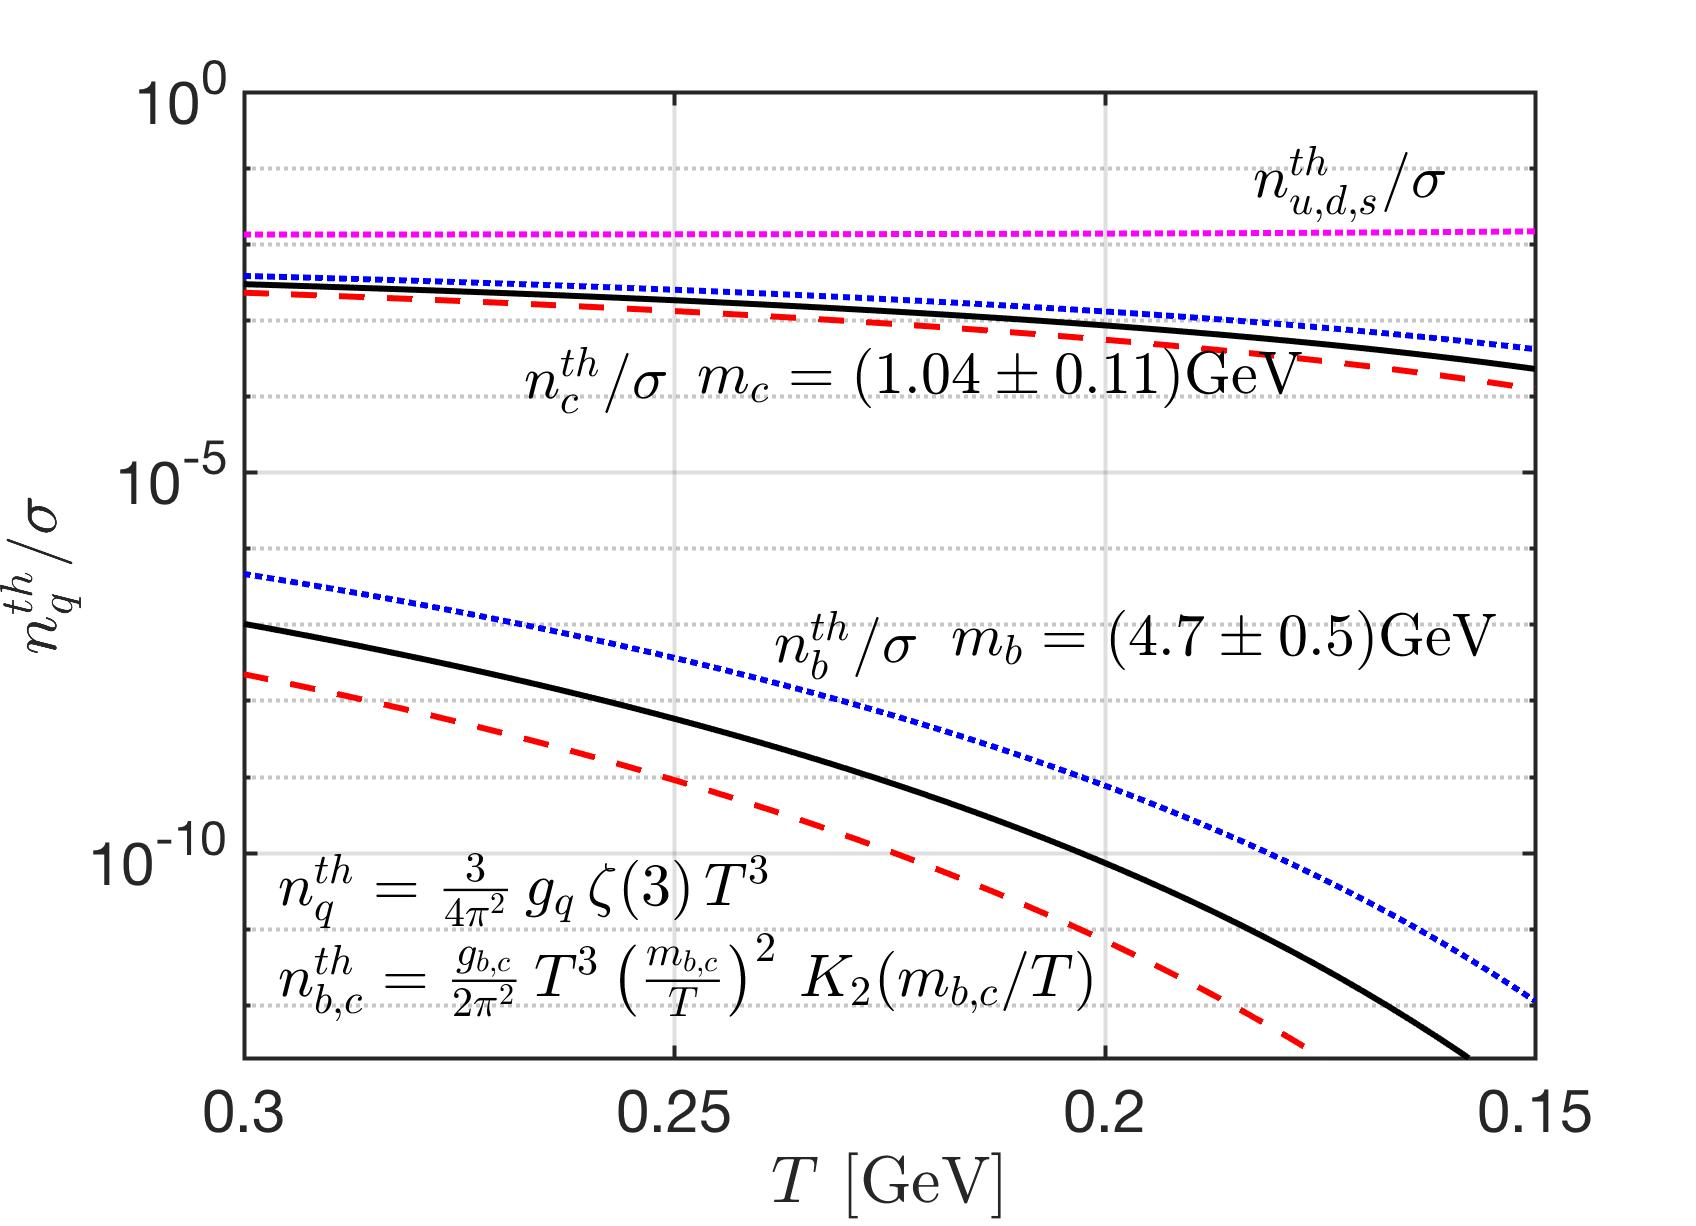
\includegraphics[width=0.9\linewidth]{./plots/bcQuarkDensity_new}}
\caption{
The equilibrium charm and bottom quark number density normalized by entropy density, as a function of temperature in the primordial Universe, see text for discussion of different mass values. \radapt{Yang:2024ret}}
\label{number_entropy_b002} 
\end{figure}
%%%%%%%%%%%%%%%%%%%%%%%%%%%%%%%%%%%%%%%%%%% 

The $m_b\simeq 5.2\,\mathrm{GeV}$ is a typical potential model mass used in modeling bound states of bottom, and $m_b=4.2,\,4.7\,\mathrm{GeV}$ is the current quark mass at low and high energy scales. In~\rf{number_entropy_b002} we see that the charm abundance in the domain of interest $0.3\,\mathrm{GeV}>T>0.15\,\mathrm{GeV}$ is about $10^4\sim 10^{9}$ times greater than the abundance of bottom quarks. This implies that the small $b$,$\bar b$ quark abundance is embedded in a large background comprising all lighter $u,d,s,c$ quarks and anti-quarks, as well as gluons $g$.

In the following we will calculate the production and decay rate for bottom and charm quarks and compare to the Universe expansion rate. We will show that in the epoch of interest to us the characteristic Universe expansion time $1/H$ is much longer than the lifespan and production time of the bottom/charm quark. In this case, the dilution of bottom/charm quark due to the Universe expansion is slow compare to the the strong interaction production, and the weak interaction decay of the bottom/charm. Any abundance nonequilibrium will therefore be nearly stationary.    

It is important for following analysis to know that the expansion of the Universe is the slowest process, allowing many microscopic reactions at a `fixed' temperature range $T$ to proceed. To show this we evaluate the Hubble\index{Hubble!parameter} relation to obtain $1/H$\,[s]
\begin{align}
H^2=\frac{8\pi G_N}{3}\left(\rho_\gamma+\rho_{\mathrm{lepton}}+\rho_{\mathrm{quark}}+\rho_{g,{W^\pm},{Z^0}}\right),
\end{align}
The effectively massless particles and radiation dominate particle energy density $\rho_i$ defining the speed of expansion of the Universe within  temperature range $130\, \mathrm{GeV}>T>0.15\,\mathrm{GeV}$; we have the following particles: photons, $8$ color charge gluons, $W^\pm$, $Z^0$, three generations of $3$ color charge quarks and leptons in the primordial QGP. The characteristic Universe expansion time constant $1/H$ is seen in~\rf{BCreaction:fig} below. In the epoch of interest to us $0.3\,\mathrm{GeV}>T>0.15\,\mathrm{GeV}$, the Hubble time $1/H\approx10^{-5}$ sec which is much longer than the microscopic lifespan and production time of the bottom and charm quarks we study 

%%%%%%%%%%%%%%%%%%%%%%%%%%%%%%%%%%%%%
\para{Quark production rate via strong interaction}\index{quark!production rate}
In primordial QGP, the bottom and charm quarks can be produced from strong interactions via quark-gluon pair fusion processes. For production, we have the following processes
\begin{align}
 q+\bar{q}&\longrightarrow b+\bar b,\qquad q+\bar{q}\longrightarrow c+\bar c,\\
 g+g&\longrightarrow b+\bar b,\qquad g+g\longrightarrow c+\bar c\,.
\end{align}

For the quark-gluon pair fusion processes\index{bottom quark!production rate}
%\begin{align}
% q+q&\longrightarrow b+\bar b,\qquad q+q\longrightarrow c+\bar c,\\
% g+g&\longrightarrow b+\bar b,\qquad g+g\longrightarrow c+\bar c,
%\end{align}
the evaluation of the lowest-order Feynman diagrams yields the cross sections~\cite{Letessier:2002ony}:
\begin{align}
&\sigma_{q\bar{q}\rightarrow b\bar{b},c\bar{c}}=\frac{8\pi\alpha_s^2}{27s}\left(1+\frac{2m_{b,c}^2}{s}\right)w(s),\,\qquad w(s)=\sqrt{1-{4m^2_{b,c}}/{s}},\\
&\sigma_{gg\rightarrow b\bar{b},c\bar{c}}=\!\frac{\pi\alpha_s^2}{3s}\bigg[\left(1\!+\!\frac{4m^2_{b,c}}{s}\!+\!\frac{m^4_{b,c}}{s^2}\right)\ln{\left(\frac{1+w(s)}{1-w(s)}\right)}\!-\!\left(\frac{7}{4}\!+\!\frac{31m^2_{b,c}}{4s}\right)w(s)\bigg],
\end{align} 
where $m_{b,c}$ represents the mass of bottom or charm quark, $s$ is the Mandelstam variable, and $\alpha_s$ is the QCD coupling constant. Considering the perturbation expansion of the coupling constant $\alpha_s$ for the two-loop approximation~\cite{Letessier:2002ony}, we have:
\begin{align}
\alpha_s(\mu^2)=\frac{4\pi}{\beta_0\ln({\mu^2/\Lambda^2})}\bigg[1-\frac{\beta_1}{\beta_0}\frac{\ln(\ln{(\mu^2/\Lambda^2)})}{\ln(\mu^2/\Lambda^2)}\bigg],
\end{align}
where $\mu$ is the renormalization energy scale and $\Lambda^2$ is a parameter that determines the strength of the interaction at a given energy scale in QCD. The energy scale we consider is based on required gluon/quark collisions above $b\bar b$ energy threshold, so we have $\mu=2m_b+T$. For the energy scale $\mu>2m_b$ we have $\Lambda=180\sim230\MeV$ ($\Lambda\approx205\MeV$ in our calculation), and the parameters $\beta_0=11-2n_f/3$, $\beta_1=102-38n_f/3$ with the number of active fermions $n_f=4$. 

%%%%%%%%%%%%%%%%%%%%%%%%%%%%%%%%%%%%%%%
\begin{figure} 
\centerline{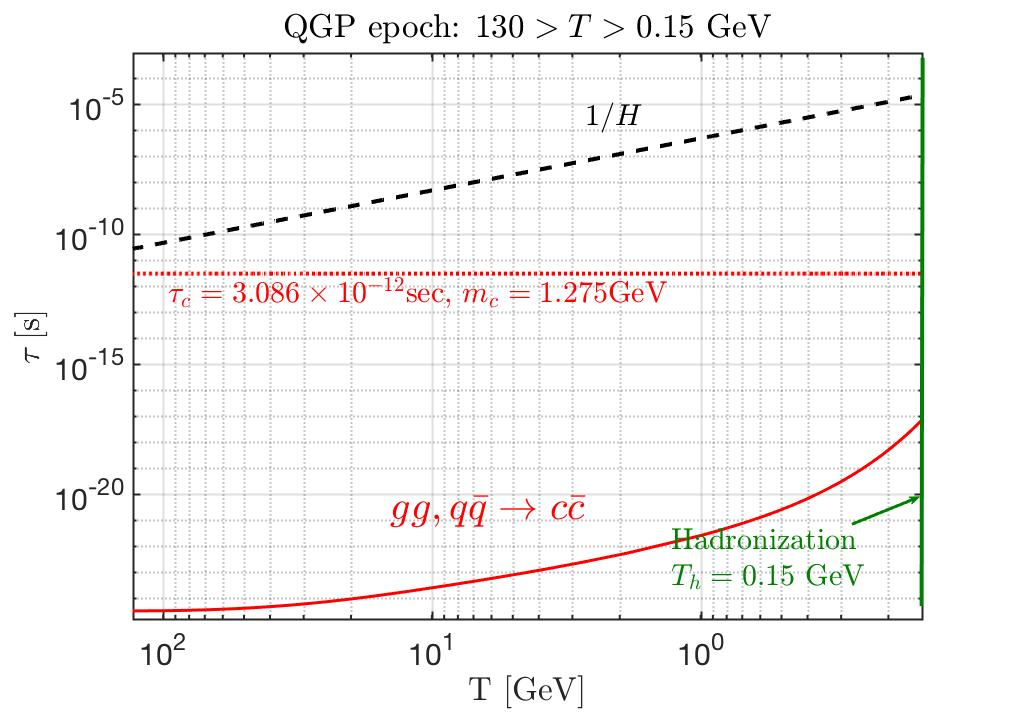
\includegraphics[width=0.9\linewidth]{./plots/CharmQuark_QGP.jpg}}
\centerline{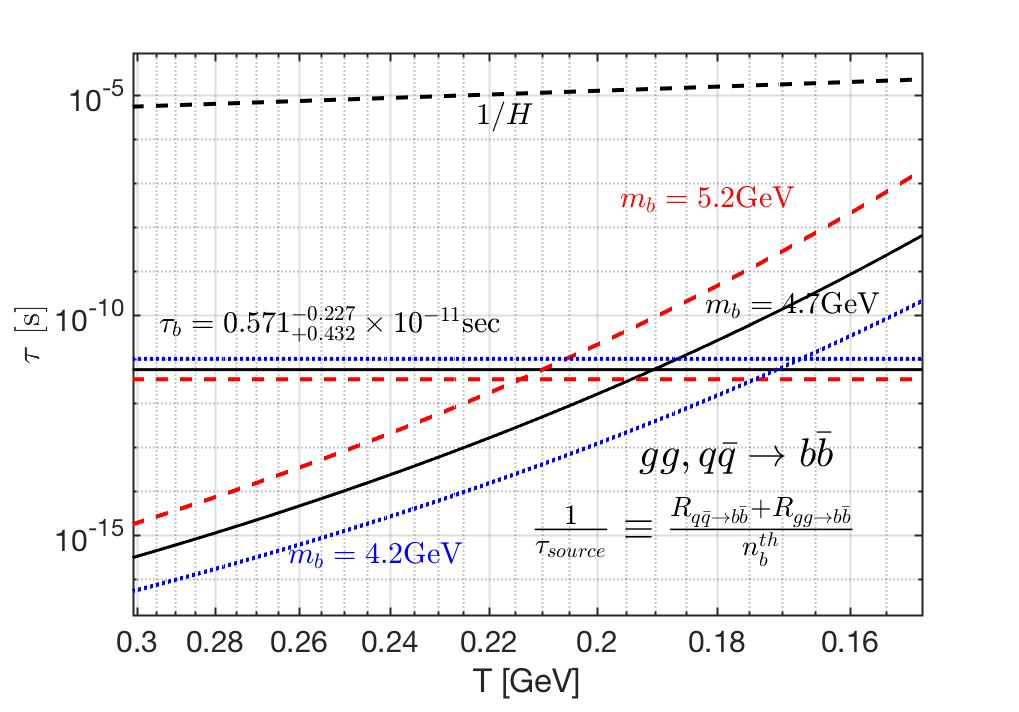
\includegraphics[width=0.9\linewidth]{./plots/BQuarkReactionTime_bottom.jpg}}
\caption{Comparison of Hubble\index{Hubble!time} time $1/H$, quark lifespan $\tau_{q}$, and characteristic time for production via quark, gluon pair fusion. The upper frame for charm $c$-quark in the entire QGP epoch $T$ rang; the lower frame for bottom $b$-quark amplifying the dynamic detail balance $T\simeq 200\MeV$. Both figures end at the hadronization temperature of $T_{H}\approx150\MeV$. See text for additional information. \cccite{Rafelski:2023emw}. \radapt{Yang:2024ret}}
\label{BCreaction:fig}
\end{figure}
%%%%%%%%%%%%%%%%%%%%%%%%%%%%%%%%%%%%%%%

In general the thermal reaction rate per unit time and volume $R$ can be written in terms of the scattering cross section as follows~\cite{Letessier:2002ony}:
\begin{align}
R\equiv\sum_i\int_{s_{th}}^\infty\!ds\,\frac{dR_i}{ds}=\sum_i\int_{s_{th}}^\infty\!ds\,\sigma_i(s)\,P_i(s),
\end{align}
where $\sigma_i(s)$ is the cross section of the reaction channel $i$, and $P_i(s)$ is the number of collisions per unit time and volume. Considering the quantum nature of the colliding particles (i.e., Fermi and Bose distribution)\index{Bose!distribution}\index{Fermi!distribution}  with the massless limit and chemical equilibrium\index{chemical equilibrium} condition ($\Upsilon=1$), we obtain~\cite{Letessier:2002ony}
\begin{align}
&P_i(s)=\frac{g_1g_2}{32\pi^4}\,\frac{T}{1+I_{12}}\frac{\lambda_2}{\sqrt{s}}\!\sum_{l,n=1}^{\infty}\!(\pm)^{l+n}\frac{K_1(\sqrt{lns}/T)}{\sqrt{ln}},\\
&\lambda_2\equiv\left[s-\left(m_1+m_2\right)^2\right]\,\left[s-\left(m_1-m_2\right)^2\right],
\end{align}
where $+$ is for boson and $-$ is for fermions, and the factor $1/(1+I_{12})$ is introduced to avoid double counting of indistinguishable pairs of particles. $I_{12}=1$ for identical pair of particles, otherwise $I_{12}=0$. Hence the total thermal reaction rate per volume for bottom quark production can be written as
\begin{align}
\label{Bquark_Source}
R^{\mathrm{Source}}_{b,c}=\int^\infty_{s_{th}}ds\,\bigg[\sigma_{q\bar{q}\rightarrow b\bar{b},c\bar{c}}\,P_q+\sigma_{gg\rightarrow b\bar{b},c\bar{c}}\,P_g\bigg]%=R_{q\bar{q}\rightarrow b\bar{b},c\bar{c}}+R_{gg\rightarrow b\bar{b},c\bar{c}}.
\end{align}
We introduce the bottom/charm quark relaxation time for the quark-gluon pair fusion as follows:
\begin{align}
\label{relaxation_time}
&{\tau_{b,c}^{\mathrm{Source}}}\equiv\frac{dn_{b,c}/d\Upsilon_{b,c}}{R^{\mathrm{Source}}_{b,c}}\;,\quad
\end{align}
where $dn_{b,c}/d\Upsilon_{b,c}=n^{th}_{b,c}$ in the Boltzmann\index{Boltzmann!approximation} approximation. The relaxation time is on the order of magnitude of time needed to reach chemical equilibrium. 

In~\rf{BCreaction:fig} we show the characteristic time for $b$ and $c$ quark strong interaction production. The $c$ quark (upper frame) is shown in the entire QGP temperature range. We note the vast 15 orders of magnitude difference between the Hubble time and the rate of production. This means that there will be very many microscopic cycles of charm production decay erasing any non-stationary effect.  For $b$ (lower frame) we restrict the view to temperature range in the domain of interest, $ 0.3\,\mathrm{GeV}>T> 0.15\,\mathrm{GeV}$. Three different masses $m_{b}=4.2\GeV$ (blue short dashes), $4.7\GeV$, (solid black), $5.2\GeV$ (red long dashes) for bottom quarks are shown. 
 
%%%%%%%%%%%%%%%%%%%%%%%%%%%%%%%%
\para{Quark decay rate via weak interaction}\index{quark!weak decay rate}
The bottom/charm quark decay via the weak interaction \index{bottom quark!decay rate} 
\begin{align}
 &b\longrightarrow c+l+\overline{\nu_l}, \qquad b\longrightarrow c+q+\bar{q},\\
&c\longrightarrow s+l+\overline{\nu_l},\qquad c\longrightarrow s+q+\bar{q}\,.
\end{align}
The vacuum decay rate for $1\to2+3+4$ in vacuum can be evaluated via the weak interaction:
\begin{align}
\frac{1}{\tau_1}=&\frac{64G^2_F\,V^2_{12}\,V^2_{34}}{(4\pi)^3g_1}\,m^5_1\times\left[\frac{1}{2}{\left(1-\frac{m^2_2}{m^2_1}-\frac{m^2_3}{m^2_1}+\frac{m^2_4}{m^2_1}\right)}\mathcal{J}_1-\frac{2}{3}\mathcal{J}_2\right],
\end{align}
where the Fermi constant is $G_F=1.166\times10^{-5}\,\mathrm{GeV}^{-2}$, $V_{ij}$ is the element of the Cabibbo-Kobayashi-Maskawa (CKM) matrix~\cite{Czarnecki:2004cw}\index{CKM matrix} for quark channel and $V_{l\nu_l}=1$ for lepton channel. The functions $\mathcal{J}_1$ and $\mathcal{J}_2$ are given by
\begin{align}
&\mathcal{J}_1\!=\!\!\!\int_0^{(1-m^2_2/m^2_1)/2}\!\!\!\!\!\!\!\!dx\left(1\!-\!2x\!-\!\frac{m^2_2}{m_1^2}\right)^{\!\!2}\left[\frac{1}{(1-2x)^2}-1\right]\\
&\mathcal{J}_2\!=\!\!\!\int_0^{(1-m^2_2/m^2_1)/2}\!\!\!\!\!\!\!\!dx\left(1\!-\!2x\!-\!\frac{m^2_2}{m_1^2}\right)^{\!\!3}\left[\frac{1}{(1-2x)^3}-1\right]
\end{align}
The modification due to the heat bath(plasma) is small because the bottom and charm mass $m_{b,c}\gg T$~\cite{Kuznetsova:2008jt}. In the temperature range we are interested in, the decay rate in the vacuum is a good approximation for our calculation. 

We show the lifespan for bottom and charm quarks in~\rf{BCreaction:fig}. For charm (upper frame) the decay is always much slower compared to production. This assures that the strong interaction processes can maintain equilibrium easily. Thus during the entire era of QGP charm quarks can be assumed to be in equilibrium condition. 

After hadronization\index{hadrons!hadronization}, charm quarks form heavy mesons that decay into several hadronic particles. The daughter particles from charm meson decay can interact and re-equilibrate within the hadron plasma. There are very many branching reactions and some involve production of only light particles. In this case the energy required to drive inverse reaction to produce heavy charm mesons is difficult to overcome. We believe this is causing the charm quark to vanish from the inventory shortly after hadronization but a detailed study has not been carried out due to complexity of the situation. 

Looking at the lower frame in~\rf{BCreaction:fig} we see that  in the case of bottom quarks the decay crosses the production rate, and this happens within QGP near to $T=200\MeV$. The intersection implies that the bottom quark\index{bottom quark} freeze-out from the primordial plasma before hadronization as the production process slows down at low temperatures and the subsequent weak interaction decay leads to a dilution of the bottom quark content within the QGP plasma. All of this occurs with rates significantly faster than Hubble expansion and thus as the Universe expands, the system departs from  chemical equilibrium in near stationary manner, because of the competition between decay and production reactions in QGP. We will show how the dynamic equation cause  the distribution to deviate from equilibrium with $\Upsilon\neq1$ in the temperature range below the crossing point but before the hadronization. 

%%%%%%%%%%%%%%%%%%%%%%%%%%%%
\subsection{Is baryogenesis possible in QGP phase?}\label{Bottom}
%%%%%%%%%%%%%%%%%%%%%%%%%%%%%%%%%%%%%%%%%%%%
\index{quark!bottom nonequilibrium}
\para{Bottom quark abundance nonequilibrium}
The competition between weak interaction decay and strong interaction production rates can lead to a nonequilibrium dynamic heavy quark abundance. We explore as example the case of bottom quarks in QGP. Similar considerations apply to all heavier PP-SM particles including in particular Higgs, W,Z gauge bosons, top $t$ quark. However, the case of $b$-quarks attracted our attention early on in context of baryogenesis since there is strong known CP violation\index{CP violation} also present.
 
The dynamic equation for bottom quark abundance in QGP can be written as \index{bottom quark!population equation}
\begin{align}
\label{Bquark_eq}
\frac{1}{V}\frac{dN_b}{dt}=\big(\,1-\Upsilon^2_{b}\,\big)\,R^{\mathrm{Source}}_{b}-\Upsilon_b\,R^{\mathrm{Decay}}_{b}\;,
\end{align}
where $R^{\mathrm{Source}}_{b}$ and $R^{\mathrm{Decay}}_{b}$ are the thermal reaction rates per volume of production and decay of bottom quark, respectively. The bottom source rates are the gluon and quark fusion rates \req{Bquark_Source}. The decay rate depends on whether the bottom quarks are freely present in the plasma or are bounded within mesons. We consider two extreme scenarios for the bottom quark population: 1.) all bottom flavor is free, and 2.) all bottom flavor is bounded into mesons in QGP. In~\rf{ReactionTime} we show the characteristic interaction times relevant to the abundance of bottom quarks, as well as the Hubble time $1/H$ for the temperature range of interest, $0.3\,\mathrm{GeV}> T> 0.15\,\mathrm{GeV}$.

%%%%%%%%%%%%%%%%%%%%%%%%%%%%%%%%%%%%%%
\begin{figure} 
\centerline{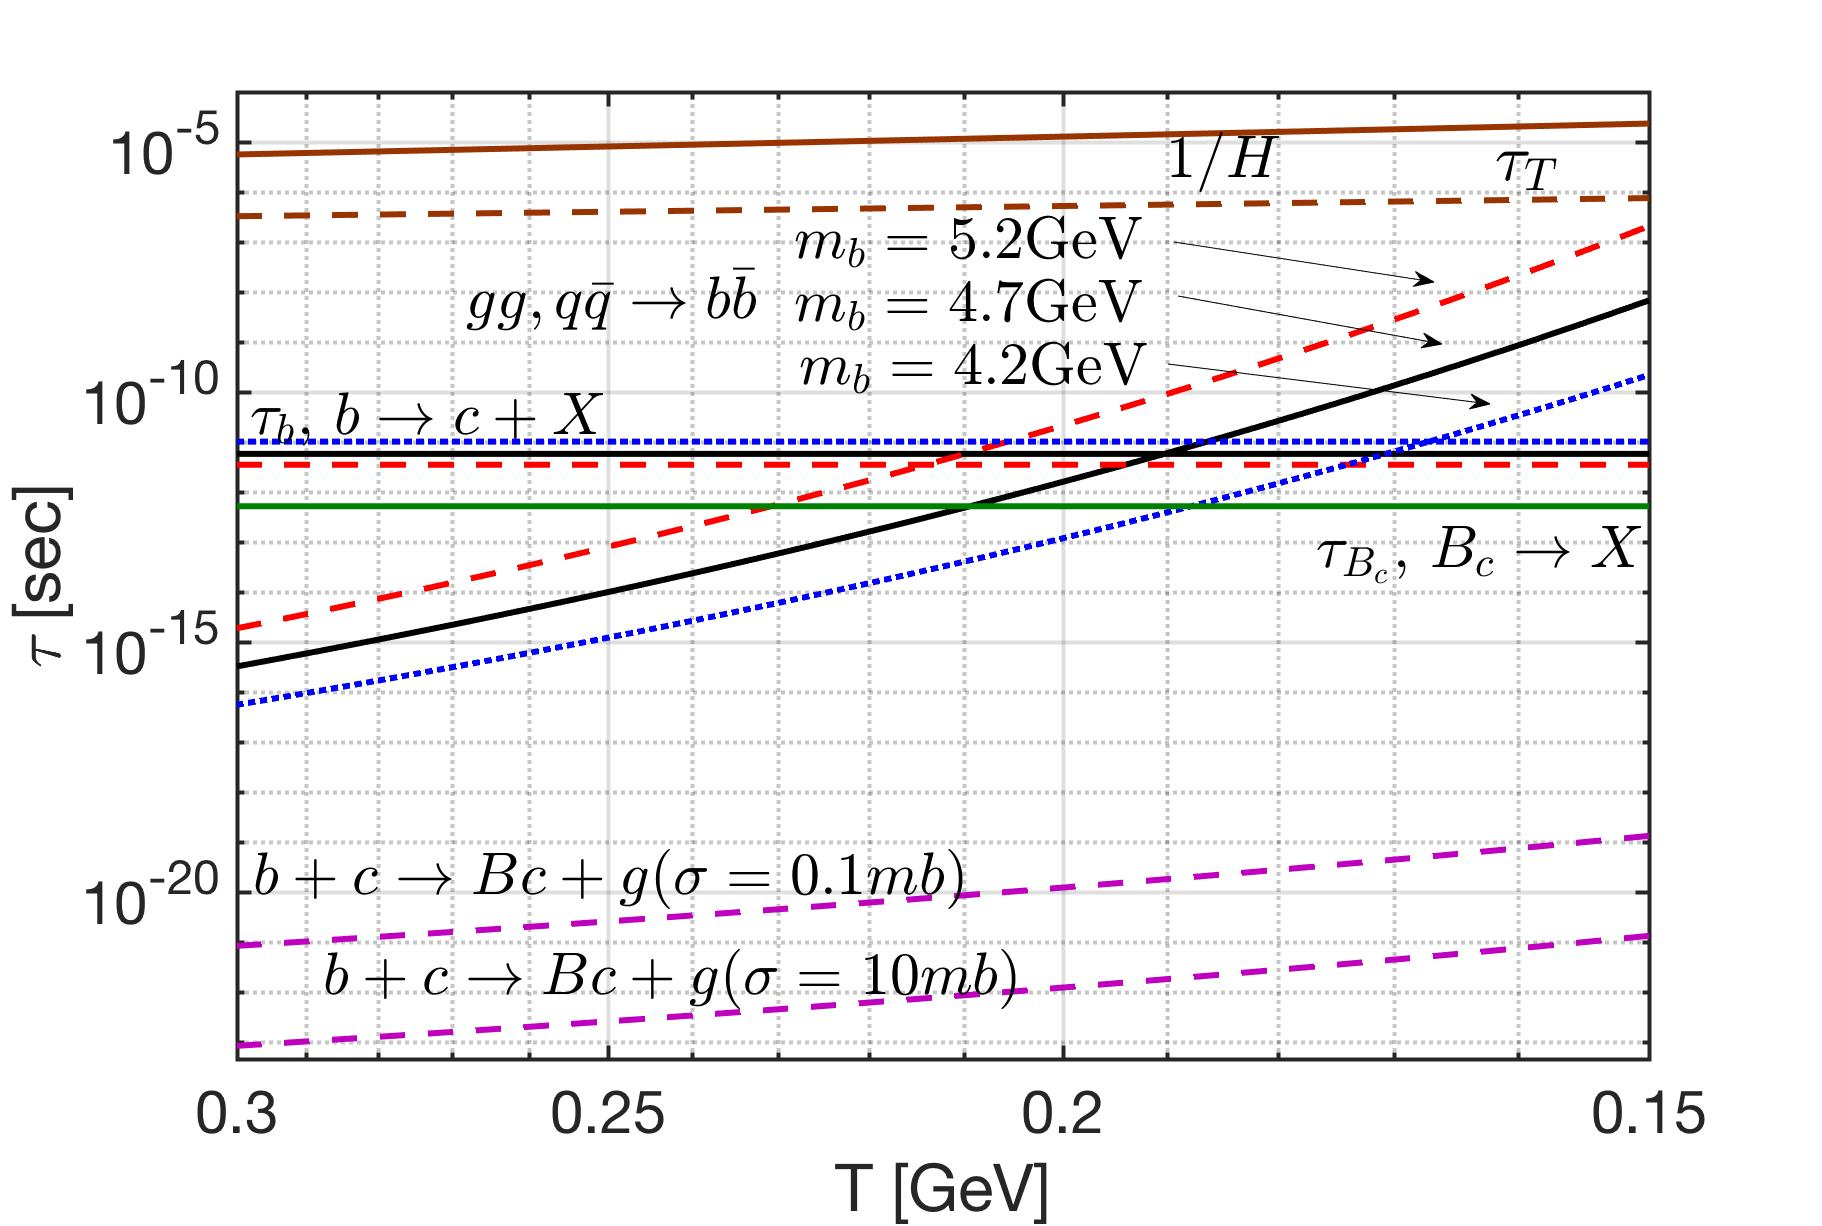
\includegraphics[width=0.9\linewidth]{./plots/BQuarkReactionTime003}}
\caption{Characteristic production, decay, times of bottom quark as a function of temperature $T$ for $0.3\,\mathrm{GeV}>T> 0.15\MeV$. Near the top of figure $1/H$ (brown solid line) and $\tau_T$ (brown dashed line); other horizontal lines are bottom-quark (in QGP) weak interaction lifetimes $\tau_b$ for the three different masses: $m_b=4.2\,\mathrm{GeV}$ (blue dotted line), $m_b=4.7\,\mathrm{GeV}$ (black solid line), $m_b=5.2\,\mathrm{GeV}$ (red dashed line), and the vacuum lifespan $\tau_B$ of the B$_c$ meson (green solid line). The relaxation time for strong interaction bottom production $g+g, q+\bar q\rightarrow b+\bar{b}$ is shown with three different bottom masses and same type-color coding as weak interaction decay rate. At bottom of figure the in plasma formation process (dashed lines, purple) $b+c\rightarrow \mathrm{B}_c+g$ with cross section range $\sigma=0.1,10\,\mathrm{mb}$. \radapt{Yang:2024ret}}
\label{ReactionTime}
\end{figure}
%%%%%%%%%%%%%%%%%%%%%%%%%%%%%%%%%

Considering all bottom flavor is free in QGP, the bottom decay rate per volume is the bottom lifespan weighted with density of particles \req{BoltzN}, see Ref.\,\cite{Kuznetsova:2008jt}. We have
\begin{align}\hspace{0.5cm}
R^{\mathrm{Decay}}_b=\frac{dn_b/d\Upsilon_b}{\tau_b},\,\,\,\,\, \tau_b\approx0.57\times10^{-11} \mathrm{sec}.
\end{align}
On the other hand, $b$,\,$\bar b$ quark abundance is embedded in a large background comprising all lighter quarks and anti-quarks (see~\rf{number_entropy_b002}). After formation the heavy $b,\,\bar b$ quark can bind with any of the available lighter quarks, with the most likely outcome being a chain of reactions 
\begin{align}
&b+q\longrightarrow\mathrm{B}+g\;,\\
&\mathrm{B}+s\longrightarrow\mathrm{B}_s+q\;,\\
&\mathrm{B}_s+c\longrightarrow\mathrm{B}_c+s\;,
\end{align}
with each step providing a gain in binding energy and reduced speed due to the diminishing abundance of heavier quarks $s, c$. To capture the lower limit of the rate of $\mathrm{B}_c$ production we show in~\rf{ReactionTime} the expected formation rate by considering the direct process $b+\overline c\rightarrow \mathrm{B}_c+g$, considering the range of cross section $\sigma=0.1\sim10\,\mathrm{mb}$ ~\cite{Schroedter:2000ek}. The rapid formation rate of B$_c(b\bar c)$ states in primordial plasma is shown by purple dashed lines at bottom in~\rf{ReactionTime}, we have
\begin{align}
\tau (b+\overline c\rightarrow \mathrm{B}_c+g)\approx(10^{-16}\sim10^{-14})\times\frac{1}{H} \;.
\end{align}

Despite the low abundance of charm, the rate of $\mathrm{B}_c$ formation is relatively fast, and that of lighter flavored B-mesons is substantially higher. Note that as long as we have bottom quarks made in gluon/quark fusion bound practically immediately with any quarks $u, d, s$ into B-mesons, we can use the production rate of $b, \bar b$ pairs as the rate of B-meson formation in the primordial-QGP, which all decay with lifespan of pico-seconds. We believe that this process is fast enough to allow consideration of bottom decay from the B$_c(b\bar c)$, $\overline{\mathrm{B}}_c(\bar b c)$ states~\cite{Yang:2020nne}. 
 
Based on the hypothesis that all bottom flavor is bound rapidly into $\mathrm{B}_c^\pm$ mesons, we have 
\begin{align}\label{Bc_source}
g+g, q+q \longleftrightarrow &b+\bar b\;[b(\bar{b})+\bar{c}(c)]\longrightarrow \mathrm{B}_c^\pm\longrightarrow\mathrm{anything}.
\end{align}
In this case, the decay rate per volume can be written as
\begin{align}\hspace{0.5cm}
 R^{\mathrm{Decay}}_b=\frac{dn_b/d\Upsilon_b}{\tau_{\mathrm{B}_c}},\,\,\,\,\, \tau_{\mathrm{B}_c}\approx0.51\times10^{-12} \mathrm{sec}.
 \end{align}


%%%%%%%%%%%%%%%%%%%%%%%%%%%%%%%
\para{Stationary and non-stationary deviation from equilibrium}
To investigate the nonequilibrium phenomena of bottom quarks, we aim to replace the variation of particle abundance seen on LHS in \req{Bquark_eq} by the time variation of abundance fugacity\index{fugacity} $\Upsilon$.
This substitution allows us to derive the dynamic equation for the fugacity parameter and enables us to study the fugacity as a function of time. Considering the expansion of the Universe we have
\begin{align}\label{number_dilution}
\frac{1}{V}\frac{dN_b}{dt}=\frac{dn_b}{d\Upsilon_b}\frac{d\Upsilon_b}{dt}+\frac{dn_b}{dT}\frac{dT}{dt}+3Hn_b,\;
\end{align}
where we use $d\ln(V)/dt=3H$ for the Universe expansion. Substituting \req{number_dilution} into \req{Bquark_eq} and dividing both sides of equation by $dn_b/{d\Upsilon_b}=n^{th}_b$, the fugacity equation becomes
\begin{align}
\frac{d\Upsilon_b}{dt}+&3H\Upsilon_b+\Upsilon_b\frac{dn^{th}_b/dT}{n^{th}_b}\frac{dT}{dt}=\left(1-\Upsilon_b^2\right)\frac{1}{\tau_{b}^{\mathrm{Source}}}-\Upsilon_b\frac{1}{\tau^{\mathrm{Decay}}_b}\;,
\end{align}
where relaxation time for bottom production is obtained using \req{relaxation_time}. It is convenient to introduce the relaxation time $1/\tau_T$ as follows,
\begin{align}
\frac{1}{\tau_T}\equiv-\frac{dn^{th}_b/dT}{n^{th}_b}\frac{dT}{dt},
\end{align}
where we put '$-$' sign in the definition to have $\tau_T>0$. The relaxation time $\tau_T$ represents how the bottom density changes due to the Universe temperature cooling. In this case, the fugacity equation can be written as
\begin{align}\label{Fugacity_Eq0}
\frac{d\Upsilon_b}{dt}\!\!=&(1-\Upsilon_{b}^2)\frac{1}{\tau_{b}^{\mathrm{Source}}}
\!-\!\Upsilon_{b}\left(\frac{1}{\tau^{\mathrm{Decay}}_b}+3H\!-\!\frac{1}{\tau_T}\right).
\end{align}
In following sections we will solve the fugacity differential equation in two different scenarios: stationary and non-stationary Universe.

%%%%%%%%%%%%%%%%%%%%%%%%%%%%%%%%%%%%%%%%%%%
In~\rf{BCreaction:fig} (bottom) we show that the relaxation time for both production and decay are faster than the Hubble\index{Hubble!time} time $1/H$ for the duration of QGP, which implies that $H,1/\tau_T\ll1/\tau_{b}^{\mathrm{Source}},1/\tau^{\mathrm{Decay}}_b$. In this scenario, we can solve the fugacity equation by considering the stationary Universe first, i.e., the Universe is not expanding and we have
\begin{align}\label{stationary}
H=0,\qquad 1/\tau_T=0.
\end{align} 
In the stationary Universe at each given temperature we consider the dynamic equilibrium condition (detailed balance)\index{detailed balance} between production and decay reactions that keep
\begin{align}
\frac{d\Upsilon_b}{dt}=0.
\end{align}
Neglecting the time dependence of the fugacity $d\Upsilon_b/dt$ and substituting the condition \req{stationary} into the fugacity equation \req{Fugacity_Eq0}, then we can solve the quadratic equation to obtain the stationary fugacity as follows: %\index{bottom quark!stationary fugacity}
\begin{align}
\label{Fugacity_Sol}
\Upsilon_{\mathrm{st}}&=\sqrt{1+\left(\frac{\tau_{source}}{2\tau_{decay}}\right)^2}-\left(\frac{\tau_{source}}{2\tau_{decay}}\right).
\end{align} 

%%%%%%%%%%%%%%%%%%%%%%%%%%%%%%%%%%%%%%
\begin{figure} 
\centerline{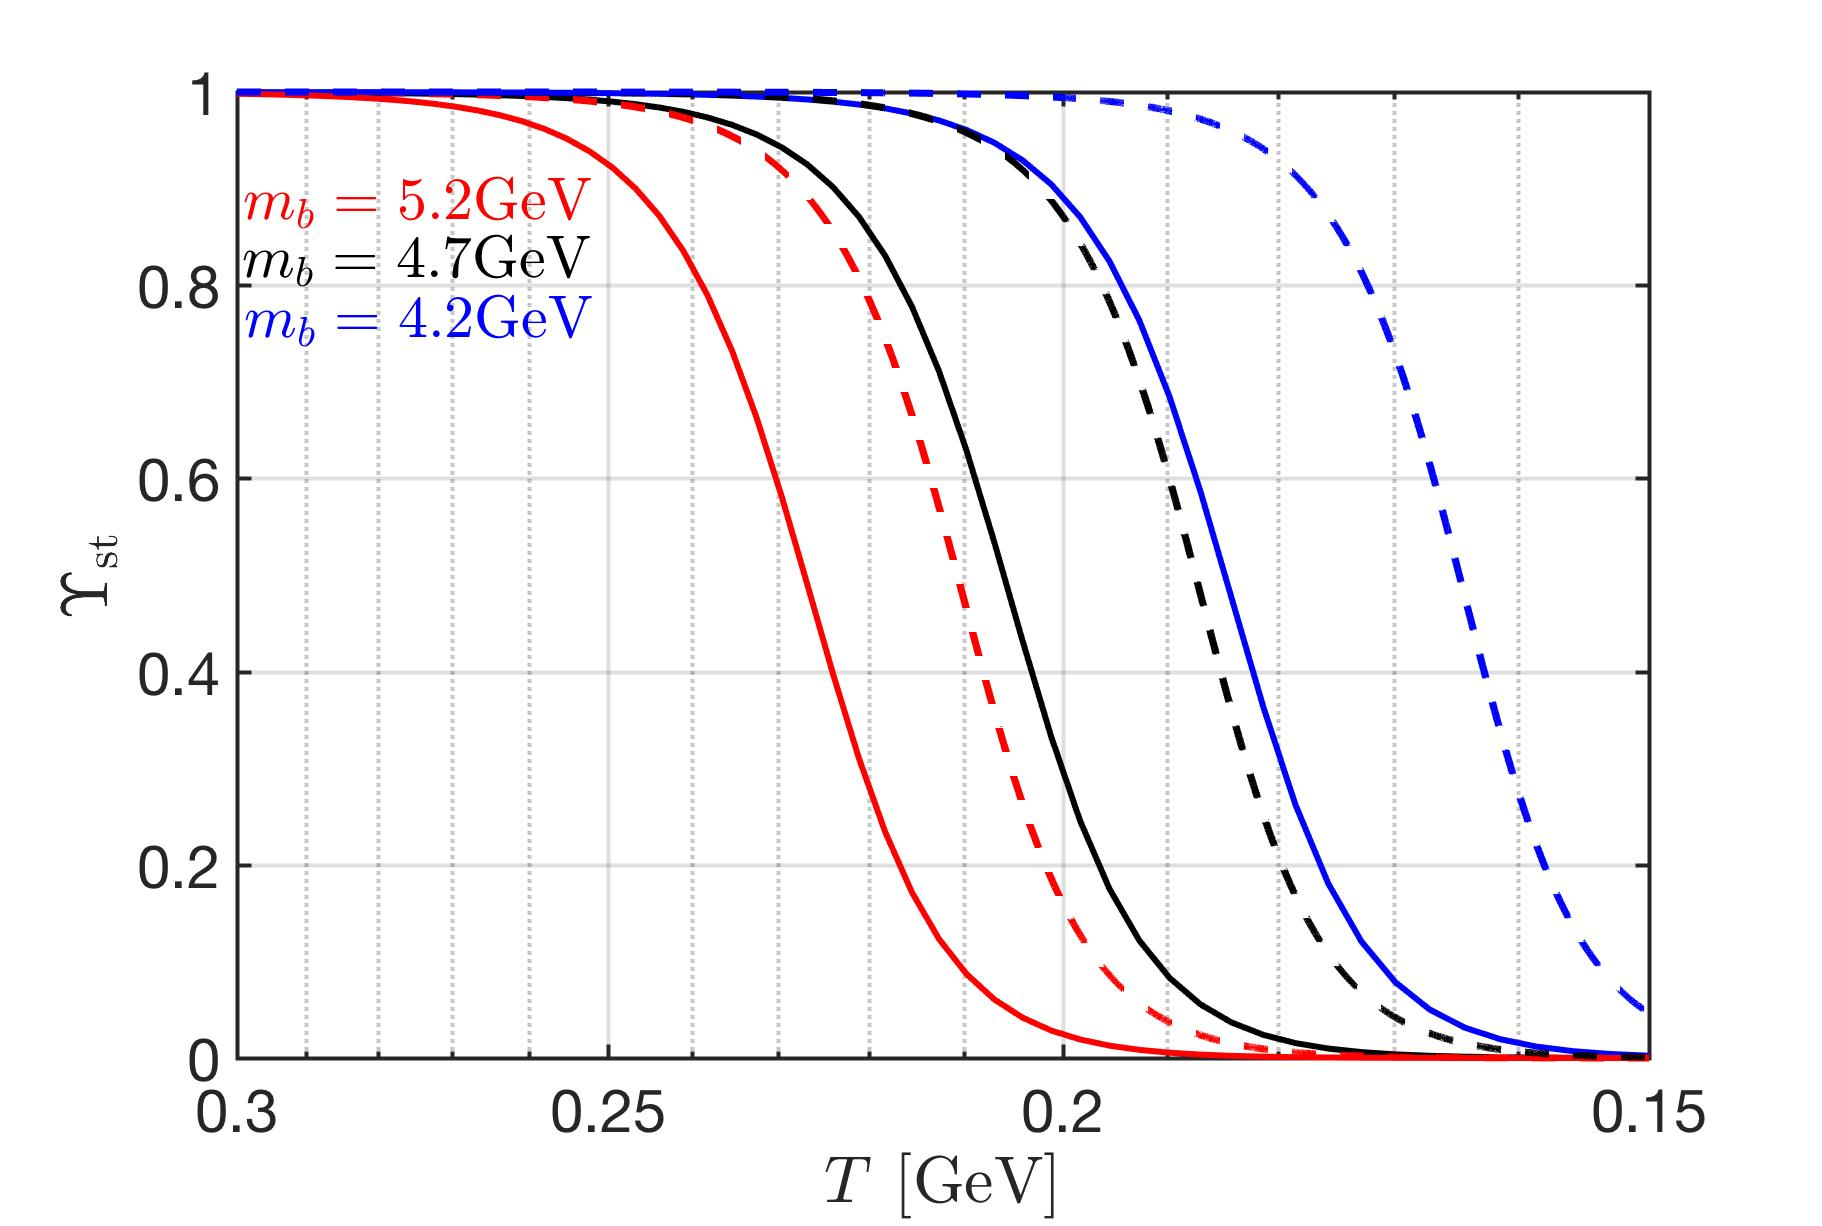
\includegraphics[width=0.9\linewidth]{./plots/BquarkFugacity_tot}}
\caption{Dynamical fugacity of bottom quark as a function of temperature in primordial Universe. Solid line shows bottom quark bound into $B_c$, dashed lines the case of free bottom quark: $m_b=4.2\,\mathrm{GeV}$ (blue), $m_b=4.7\,\mathrm{GeV}$ (black), and $m_b=5.2\,\mathrm{GeV}$ (red). \cccite{Rafelski:2023emw}. \radapt{Yang:2024ret}}
\label{fugacity_bc}
\end{figure}
%%%%%%%%%%%%%%%%%%%%%%%%%%%%%%%%%%%%%%%%%

In~\rf{fugacity_bc} the fugacity of bottom quark\index{bottom quark} $\Upsilon_{\mathrm{st}}$ as a function of temperature, \req{Fugacity_Sol} is shown around the temperature $T=0.3\,\mathrm{GeV}>T>0.15\,\mathrm{GeV}$ for different masses of bottom quarks. In all cases we see prolonged nonequilibrium, this happens since the decay and reformation rates of bottom quarks are comparable to each other as we have noted in~\rf{ReactionTime} where both lines cross. One of the key results shown in~\rf{fugacity_bc} is that the smaller mass of bottom quark slows the strong interaction formation rate to the value of weak interaction decays just near the phase transformation of QGP to HG phase. Finally, the stationary fugacity corresponds to the reversible reactions in the stationary Universe. In this case, there is no arrow in time for bottom quark because of the detailed balance.

We now consider non-stationary correction in expanding Universe allowing for the Universe expanding and thus temperature being a function of time. This leads to non-stationary correction related to time dependent fugacity in the expanding Universe. 

In general, the fugacity of bottom quark can be written as 
\begin{align}\label{Nonstationary_sol}
&\Upsilon_b=\Upsilon_{\mathrm{st}}+\Upsilon^{\mathrm{non}}_{\mathrm{st}}=\Upsilon_\mathrm{st}\left(1+x\right),\quad x\equiv{\Upsilon_\mathrm{st}^{\mathrm{non}}}/{\Upsilon_\mathrm{st}},
\end{align}
where the variable $x$ corresponds to the correction due to non-stationary Universe. Substituting the general solution \req{Nonstationary_sol} into differential equation \req{Fugacity_Eq0}, we obtain
\begin{align}\label{Nonstationary_eq}
\frac{dx}{dt}=-x^2\frac{\Upsilon_\mathrm{st}}{\tau_{source}}&-x\left[\frac{1}{\tau_{eff}}+3H-\frac{1}{\tau_T}\right]-\left[\frac{d\ln\Upsilon_\mathrm{st}}{dt}+3H-\frac{1}{\tau_T}\right],
\end{align}
where the effective relaxation time $1/\tau_{eff}$ is defined as
\begin{align}
\frac{1}{\tau_{eff}}\equiv\left[\frac{2\Upsilon_\mathrm{st}}{\tau_{source}}+\frac{1}{\tau_{decay}}+\frac{d\ln\Upsilon_\mathrm{st}}{dt}\right].
\end{align}

%%%%%%%%%%%%%%%%%%%%%%%%%%%%%%
\begin{figure} 
\centerline{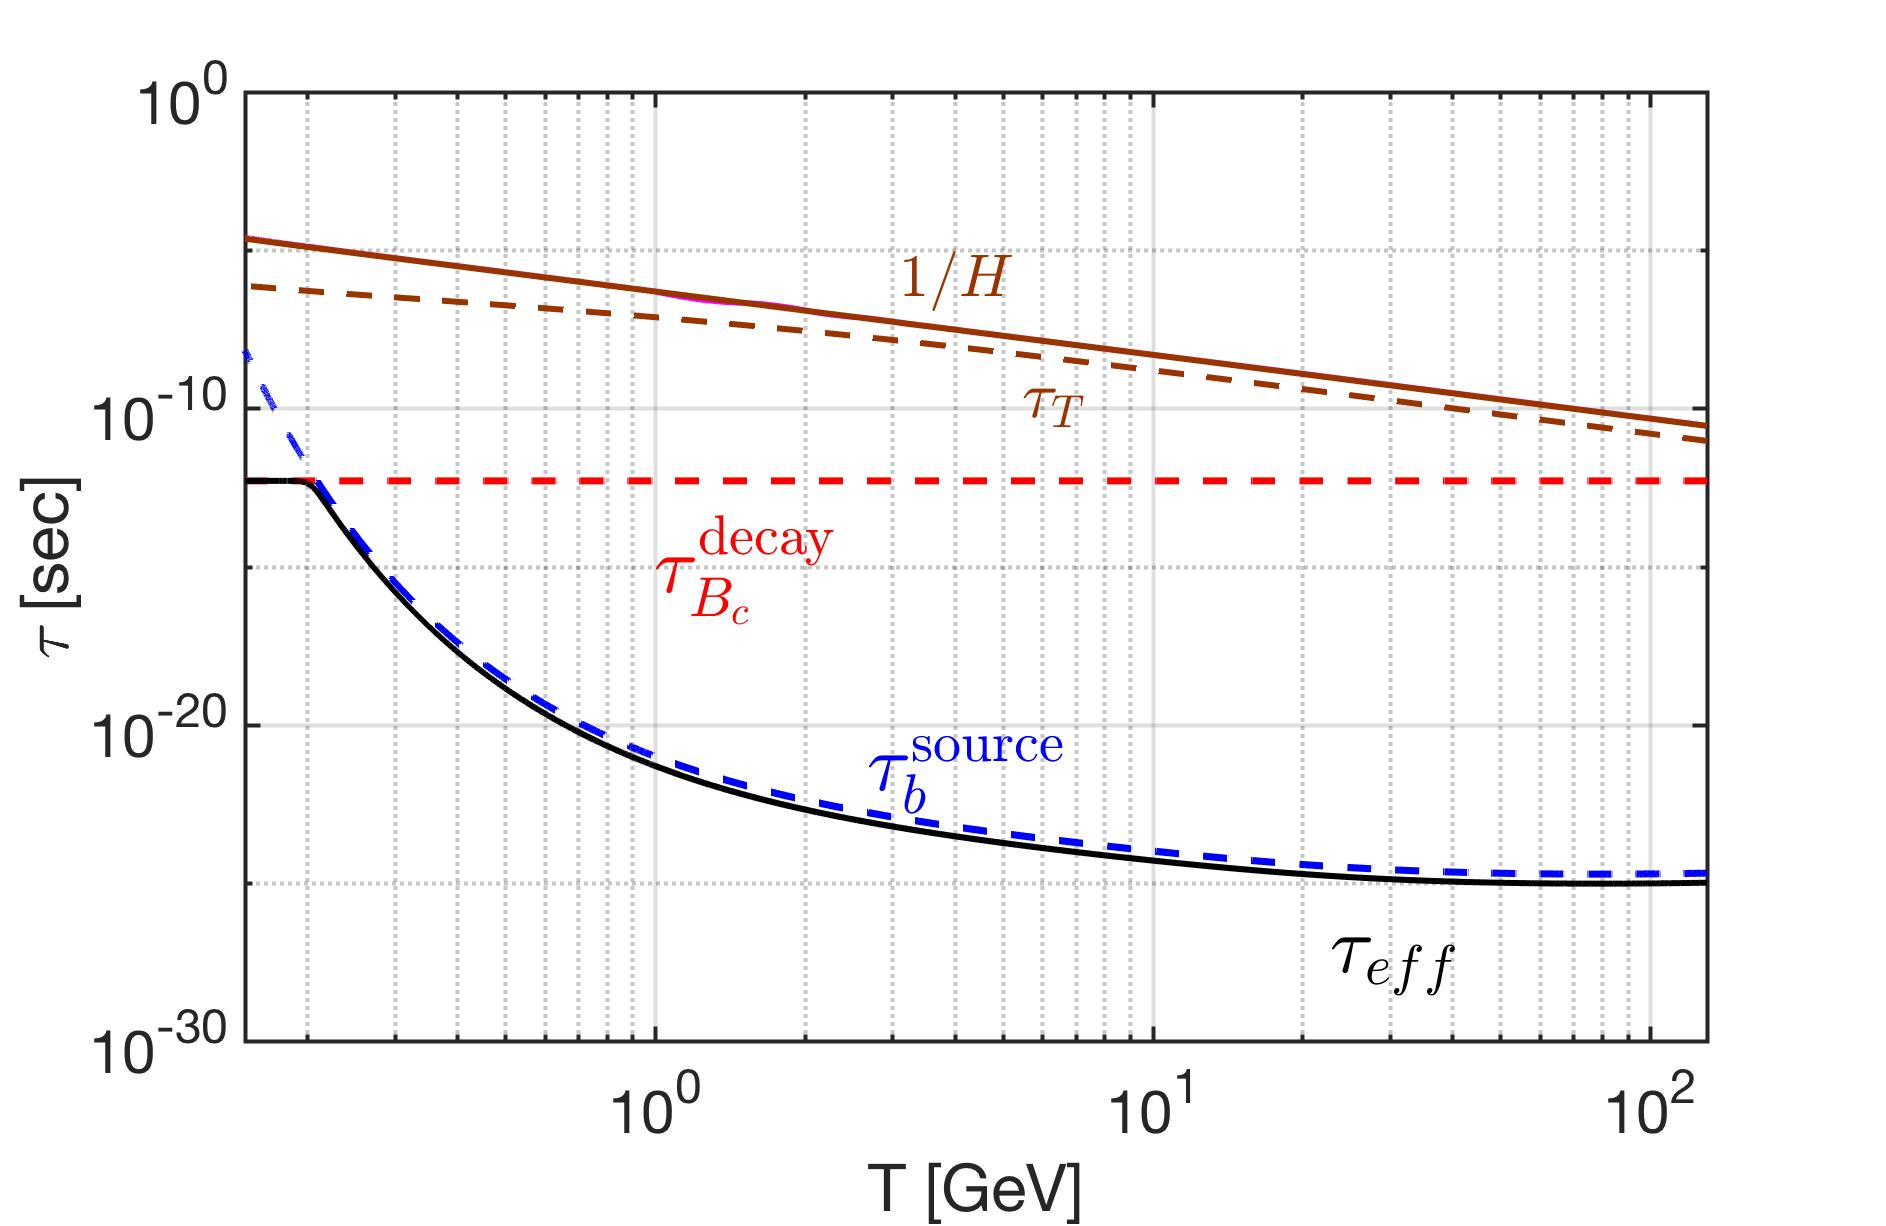
\includegraphics[width=0.9\linewidth]{./plots/Tau_RelaxationTime002}}
\caption{The effective relaxation time $\tau_{eff}$ as a function of temperature in the primordial Universe for bottom mass $m_b=4.7$\,GeV. For comparison, we also plot the vacuum lifespan of $B_c$ meson $\tau_{B_c}^{decay}$ (red dashed-line), the relaxation time for bottom production $\tau^b_{source}$ (blue dashed-line), Hubble expansion time $1/H$(brown solid line) and relaxation time for temperature cooling $\tau_T$ (brown dashed-line). \radapt{Yang:2024ret}}
\label{RelaxationTime_eff}
\end{figure}
%%%%%%%%%%%%%%%%%%%%%%%%%%%%%%%%%

In~\rf{RelaxationTime_eff} we see that when temperature is near to $T=0.2\GeV$, we have $1/\tau_{eff}\approx10^{7}H$, and $1/\tau_{eff}\approx10^5/\tau_T$. In this case, the last two terms in \req{Nonstationary_eq} compare to $1/\tau_{eff}$ can be neglected, and the differential equation becomes
\begin{align}\label{nonstationary_eq}
\frac{dx}{dt}=-\frac{x^2\,\Upsilon_\mathrm{st}}{\tau_{source}}&-\frac{x}{\tau_{eff}}-\left[\frac{d\ln\Upsilon_\mathrm{st}}{dt}+3H-\frac{1}{\tau_T}\right],
\end{align}

To solve the variable $x$ we consider the case $dx/dt,x^2\ll1$ first, we neglect the terms $dx/dt$ and $x^2$ in \req{nonstationary_eq} then solve the linear fugacity equation. We will establish that these approximations are justified by checking the magnitude of the solution. Neglecting terms $dx/dt$ and $x^2$ in \req{nonstationary_eq} we obtain
\begin{align}
x\approx\tau_{eff}\left[\frac{d\ln\Upsilon_\mathrm{st}}{dt}+3H-\frac{1}{\tau_T}\right].
\end{align}
It is convenient to change the variable from time to temperature. For an isentropically-expanding universe, we have
\begin{align}\label{tau_H}
\frac{dt}{dT}=-\frac{\tau^\ast_H}{T},\qquad \tau^\ast_H=\frac{1}{H}\left(1+\frac{T}{3g^s_\ast}\frac{dg^s_\ast}{dT}\right).
\end{align}
In this case, we have
\begin{align}
x=\tau_{eff}\left[\frac{1}{\Upsilon_\mathrm{st}}\frac{d\Upsilon_\mathrm{st}}{dT}\frac{T}{\tau^\ast_H}+3H-\frac{1}{\tau_T}\right].
\end{align}
Finally, we can obtain the non-stationary fugacity\index{fugacity} by multiplying the fugacity ratio $x$ with $\Upsilon_\mathrm{st}$, giving \index{bottom quark! non-stationary fugacity}
\begin{align}
\Upsilon_{\mathrm{st}}^{\mathrm{non}}
&\approx\left(\frac{\tau_{eff}}{\tau^\ast_H}\right)\left[\frac{d\Upsilon_\mathrm{st}}{dT}T-\Upsilon_{\mathrm{st}}\left(3H\tau^\ast_H-\frac{\tau^\ast_H}{\tau_T}\right)\right].
\end{align}

In~\rf{NonFugacity} we plot the non stationary $\Upsilon^{\mathrm{non}}_\mathrm{st}$ as a function of temperature. The non stationary fugacity $\Upsilon^{\mathrm{non}}_\mathrm{st}$ follows the behavior of $d\Upsilon_{\mathrm{st}}/dT$, which corresponds to the irreversible process in expanding Universe. In this case, the irreversible nonequilibrium process creates the arrow in time for bottom quark in the Universe. The large value of Hubble time compares to the effective relaxation time suppressing the value of non-stationary fugacity to $\mathcal{O}\sim10^{-7}$, which shows that the neglecting $dx/dt,x^2\ll1$ is a good approximation for solving the non-stationary fugacity in the primordial Universe.


%%%%%%%%%%%%%%%%%%%%%%%%%%%%%%%%%%%
\begin{figure}
\centerline{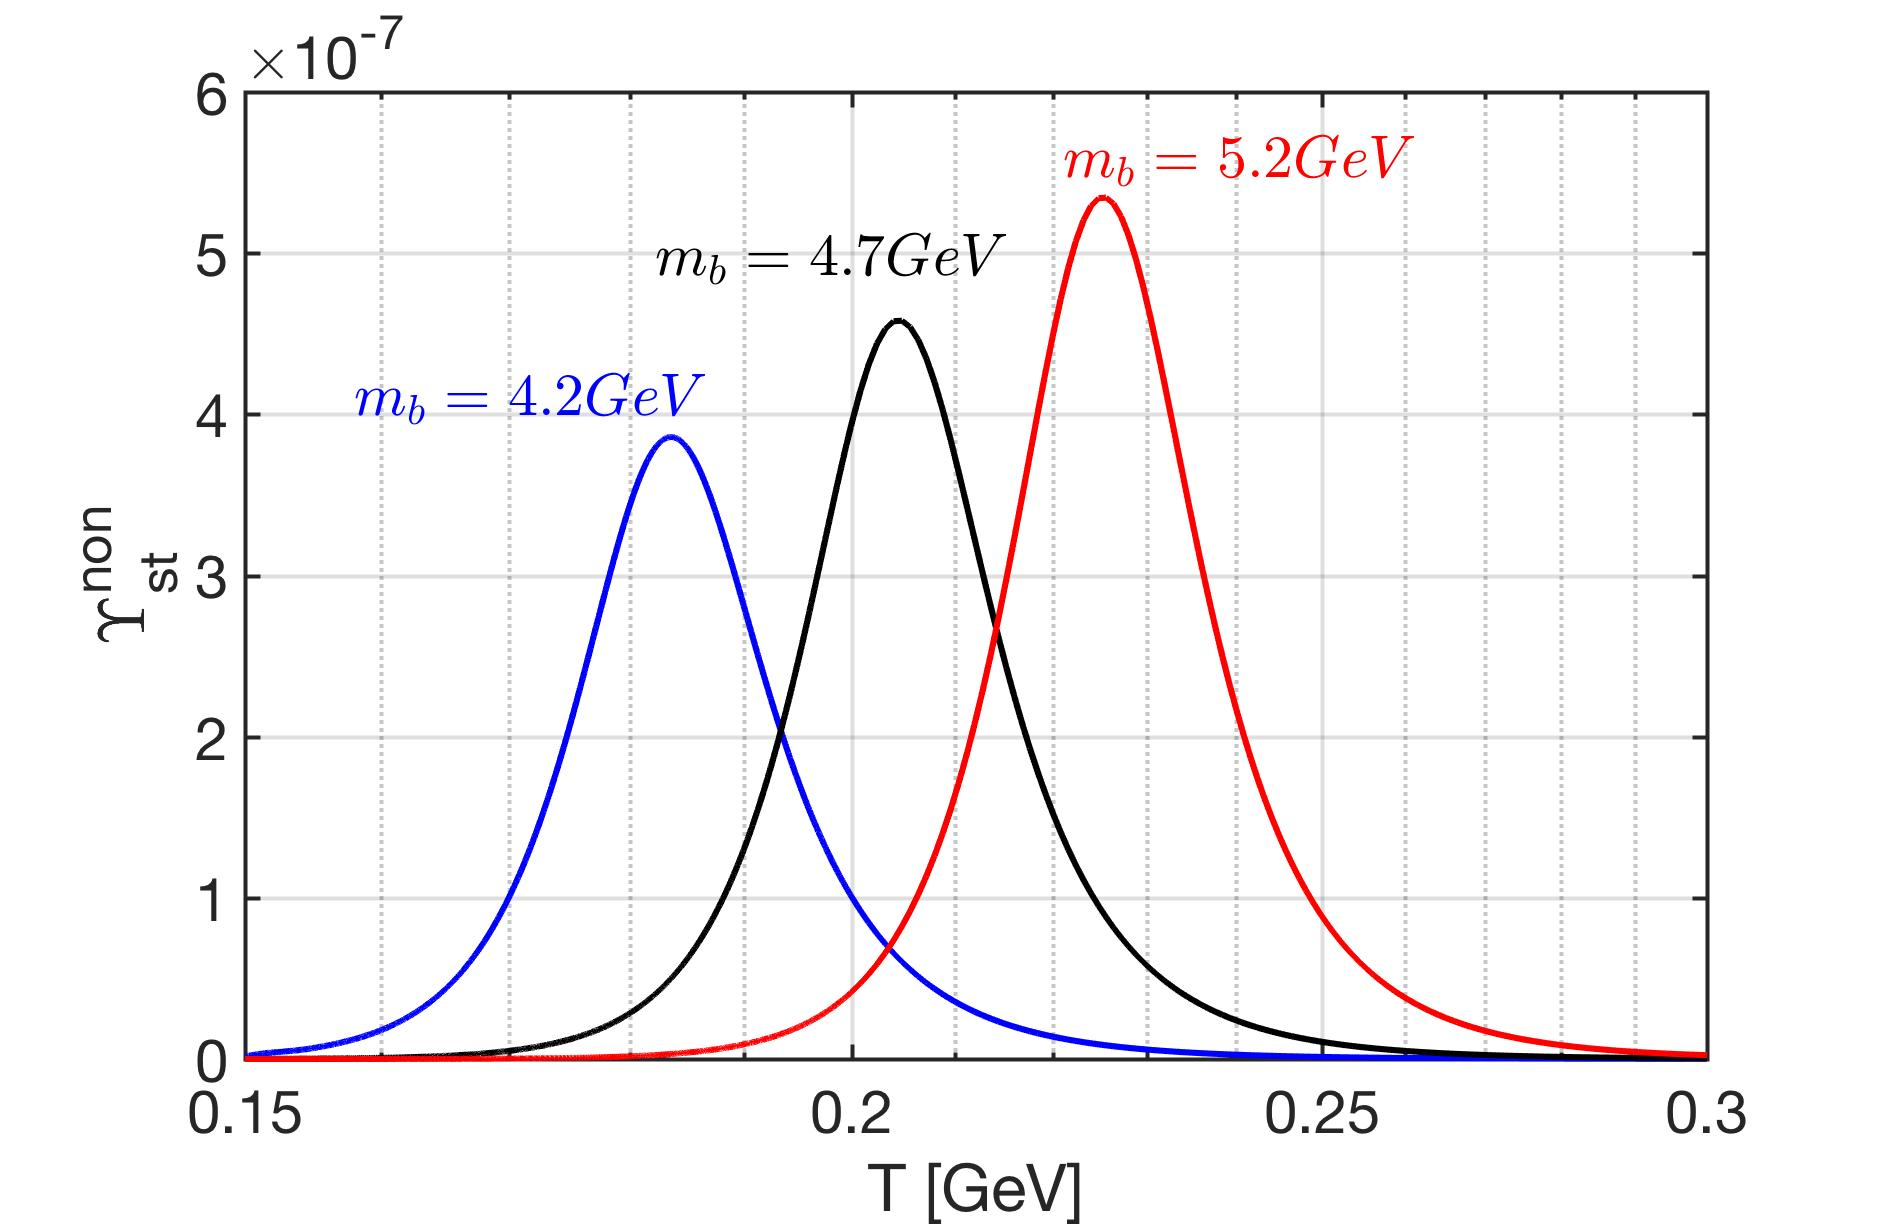
\includegraphics[width=0.9\linewidth]{./plots/NonstationaryFugacity}}
\caption{The non-stationary fugacity $\Upsilon_\mathrm{st}^{\mathrm{non}}$ as a function of temperature in the Universe for different bottom mass $m_b=4.2\,\mathrm{GeV}$ (blue), $m_b=4.7\,\mathrm{GeV}$ (black), and $m_b=5.2\,\mathrm{GeV}$ (red) for the case bottom quarks bound into $B_c$ mesons. \radapt{Yang:2024ret}}
\label{NonFugacity}
\end{figure}
%%%%%%%%%%%%%%%%%%%%%%%%%%%%%%%%%%%%%%
 

%%%%%%%%%%%%%%%%%%%%%%%%%%%%%%%%%%
\para{Is there enough bottom flavor to matter?} Considering that FLRW-Universe evolves\index{cosmology!FLRW} conserving entropy, and that baryon and lepton number following on the era of matter genesis is conserved, the current day baryon $B$ to entropy $S$, $B/S$-ratio must be achieved during matter genesis. The estimates of present day baryon-to-photon density\index{baryon!per photon ratio} ratio $\eta$ allows the determination of the present value of baryon per entropy\index{baryon!entropy ratio} ratio \cite{Rafelski:2019twp,Letessier:2002ony,Fromerth:2002wb,Fromerth:2012fe}:
\begin{align}
\left(\frac{B}{S}\right)_{t_0}\!\!\!\!=\eta\left(\frac{n_\gamma}{\sigma_\gamma+\sigma_\nu}\right)_{\!t_0}\!\!\!\!=(8.69\pm0.05)\!\!\times\!\!10^{-11},
\end{align}
where the subscript $t_0$ denotes the present day value, where $\eta=(6.12\pm0.04)\times10^{-10}$~\cite{ParticleDataGroup:2018ovx} is used in calculation. Here we consider that the Universe today is dominated by photons and free-streaming\index{free-streaming} low mass neutrinos~\cite{Birrell:2012gg}, and $\sigma_\gamma$ and $\sigma_\nu$ are the entropy density for photons and neutrinos, respectively. 
 
In chemical equilibrium\index{chemical equilibrium} the ratio of bottom quark\index{bottom quark} (pair) density $n_b^{th}$ to entropy density\index{entropy!density} $\sigma=S/V$ just above quark-gluon hadronization\index{hadrons!hadronization} temperature $T_\mathrm{H}=150\sim160\MeV$ is $n_b^{th}/\sigma=10^{-10}\sim 10^{-13}$ (see~\rf{number_entropy_b002}. By studying the bottom density per entropy near to the hadronization temperature and comparing it to the baryon-per-entropy ratio $B/S$ we found that there is sufficient abundance of bottom quarks for the proposed matter genesis mechanism to be relevant.

%%%%%%%%%%%%%%%%%%%%%%%%%%%%%%%%
\para{Example of bottom-catalyzed matter genesis}
Given that the nonequilibrium non-stationary component of bottom flavor arises at relatively low QGP temperature, this Sakharov condition is available around QGP hadronization. Let us now look back and see how different requirements are fulfilled
%%%%%%%%%%%%%%%%%%%%%%%%%%%%%%%%%%%%
\begin{itemize}
\item
 We have demonstrated non-stationary conditions with absence of detailed balance: The competition between weak interaction decay and the strong interaction gluon fusion process is responsible for driving the bottom quark departure from the equilibrium in the primordial Universe near to QGP hadronization condition around the temperature $T=0.3\sim0.15\GeV$ as shown in~\rf{fugacity_bc}. Albeit small there is clear non-stationary component required for baryogenesis, see~\rf{NonFugacity}.
%%%%%%%%%%%%%%%%%%%%%%%%%%%%%%%
\item Violation of $CP$\index{CP violation} asymmetry were observed in the amplitudes of hadron decay including neutral B-mesons, see for example~\cite{LHCb:2019jta,LHCb:2020vut}. The weak interaction $CP$ violation\index{CP violation}\index{CKM matrix} arises from the components of Cabibbo-Kobayashi-Maskawa (CKM) matrix associated with quark-level transition amplitude and $CP$-violating phase. There is clear coincidence of non stationary component of bottom yield with the bottom quark $CP$ violating decays of preformed $\mathrm{B}_x$ meson states, $x=u,d,s,c$~\cite{Karsch:1987pv,Brambilla:2010vq,Aarts:2011sm,Brambilla:2017zei,Bazavov:2018wmo,Offler:2019eij}. The exploration of the here interesting $CP$ symmetry breaking in B$_c(b\bar c)$ decay is in progress~\cite{Tully:2019ltb,HFLAV:2019otj,ParticleDataGroup:2018ovx}. % Present measurements of $CP$-violation suggest that the CP asymmetry parameter is around $\delta_{CP}\approx10^{-3}$ ~\cite{ParticleDataGroup:2018ovx}.
\item
We do not know if there is baryon\index{baryon} number violating process in which one of the heavy particles, including bottom quark, is participating. However, if such a process were to exist it is likely, considering mass thresholds, that it would be most active in the decays of heaviest standard model particles. It is thus of considerable interest to study in lepton colliders baryon number non conserving processes at resonance condition. Such a research program will additionally be motivated by our demonstration of an extended period of baryogenesis in the primordial Universe. 
\end{itemize}

%%%%%%%%%%%%%%%%%%%%


\para{Circular Urca amplification}
The off equilibrium phenomenon of bottom quark around the temperature range $T=0.3\sim0.15\GeV$ can provide the non-chemical equilibrium non-stationary condition for baryogenesis to occur in the primordial-QGP hadronization era. The processes of interest as we saw are small. However there is additional amplifying factor. 
 
 Let us consider the scenario where all bottom quarks are confined within $B_c^\pm$ meson. In this case, the decay of charged mesons in the primordial-QGP can be a source of $CP$ violation. However, it remains uncertain whether the decay of $B_c^\pm$ mesons contributes to baryon violation. Our postulation is as follows: the baryon asymmetry\index{baryon!asymmetry} is produced by the bottom quark disappearance via the irreversible decay of $B^\pm_c$ meson during the off-equilibrium process. Once a baryon symmetry exists in universe, it will also produce the asymmetry between leptons\index{lepton} and anti-leptons which is similar to the baryon asymmetry by the $L=B$.

The heavy $B_c^\pm$ meson decay into multi-particles in plasma is associated with the irreversible process. This is because after decay the daughter particles can interact with plasma and distribute their energy to other particles and reach equilibrium with the plasma quickly. In this case the energy required for the inverse reaction to produce $B_c^\pm$ meson is difficult to overcome and therefore we have an irreversible process for multi-particle decay in plasma.


The rapid $B_c^\pm$ decay and bottom reformation speed at picosecond scale assures that there are millions of individual microscopic processes involving bottom quark production and decay before and during the hadronization epoch of QGP. In this case, we have an Urca process for the bottom quark, i.e. a cycling reaction that produces the bottom quark which subsequently disappears via the $B_c^\pm$ meson decay. 

The Urca process is a fundamental physical process and has been studying the realms of in astrophysics and nuclear physics. In our case, for bottom quark as a example: at low temperature, the number of bottom quark cycling can be estimated as
\begin{align}
\left.\mathrm{C_{cycle}}\right|_{T=0.2\mathrm{GeV}}=\frac{\tau_H}{\tau_{B_c}}\approx2\times10^7,
\end{align}
where the lifespan of $B_c^\pm$ is $\tau_{\mathrm{B}_c}\approx0.51\times10^{-12}\,\mathrm{sec}$ and at temperature $T=0.2\GeV$ the Hubble\index{Hubble!time} time is $\tau_H=1/H=1.272\times10^{-5}$ sec. The Urca process plays a significant role by potentially amplifying any small and currently unobserved violation of baryon number associated with the bottom quark. The small baryon asymmetry is enhanced by the Urca-like process with cycling ${\tau^\ast_H}/{\tau_\ast}$ in the primordial Universe.
This amplification would be crucial for achieving the required strength for today's observation. 


%%%%%%%%%%%%%%%%%%%%%%%%%%%%%%%%%%%%%%%%%%%%%%%%
\subsection{Strange hadron abundance in cosmic plasma}
\label{Strangeness}\index{strangeness}
%%%%%%%%%%%%%%%%%%%%%%%%%%%%%%%%%%
\para{Hadron populations in equilibrium}
As the Universe expanded and cooled down to the QGP Hagedorn temperature\index{Hagedorn!temperature} $T_H\approx150\MeV$, the primordial QGP underwent a phase transformation called hadronization. Quarks and gluons fragmented, combined and formed matter and antimatter  we are familiar with. After hadronization\index{hadrons!hadronization}, one may think that all relatively short lived massive hadrons decay rapidly and disappear from the Universe. However, the most abundant hadrons\index{hadrons}, pions $\pi(q\bar q)$, can be produced via their inverse decay process $\gamma\gamma\rightarrow\pi^0$. Therefore they retain their chemical equilibrium  down to $T=3\sim5\MeV$~\cite{Kuznetsova:2008jt}. 

We begin by determining the Universe particle population composition assuming both kinetic and particle abundance equilibrium (chemical equilibrium) of non-interacting bosons and fermions. By considering the charge neutrality\index{charge neutrality} and a prescribed conserved baryon-per-entropy-ratio\index{baryon!entropy ratio} ${(n_B-n_{\overline{B}})}/{\sigma}$ we can  determine the baryon chemical potential\index{chemical potential!baryon} $\mu_B$~\cite{Fromerth:2002wb,Fromerth:2012fe,Rafelski:2013yka}. We extend this approach  allowing for the presence of strange hadrons, and imposing conservation of strangeness in the primordial Universe -- the  strange quark content in hadrons must equal the anti-strange quark content in statistical average $\langle s-\bar s \rangle=0$. 

Given $\mu_B(T)$, $\mu_s(T)$ the baryon and strangeness chemical potentials as a function of temperature, we can obtain the particle number densities for different strange and non-strange species and study their population in the primordial Universe. Our approach prioritizes strangeness pair production into bound hadron states by strong or electromagnetic interactions over the also possible weak interaction strangeness changing processes capable to amplify the effect of baryon asymmetry. This is another topic beyond scope of this work and deserving further attention.

To characterize the baryon and strangeness content of a hadron we employ the chemical fugacity\index{fugacity!strangeness} for strangeness $\lambda_s$ and for light quarks $\lambda_q$ \index{quark!fugacity}
\begin{align}
\lambda_s=\exp(\mu_s/T)\,\quad \lambda_q=\exp(\mu_B/3T)\,.
\end{align}
Here $\mu_s$ and $\mu_B$ are the chemical potential of strangeness and baryon, respectively. To obtain quark fugacity\index{fugacity!quark} $\lambda_q$, we divide the baryo-chemical potential of baryons by quark content in the baryon, \ie\ three.

When the baryon chemical potential does not vanish the chemical potential of strangeness in the primordial Universe is obtained imposing the conservation of strangeness constraint $\langle s-\bar s \rangle=0$, see Section 11.5 in Ref.\,\cite{Letessier:2002ony}\index{strangeness! chemical potential}
\begin{align}\label{museq}
\lambda_s=\lambda_q\sqrt{\frac{F_K+\lambda^{-3}_q\,F_Y}{F_K+\lambda^3_q\,F_Y}}\,.
\end{align}
where we employ the phase-space function $F_i$ for sets of nucleon $N$, kaons $K$, and hyperon\index{hyperon} $Y$ particles 
\begin{align}
&F_N=\sum_{N_i}\,g_{N_i}W(m_{N_i}/T)\;, \quad N_i=n, p, \Delta(1232),\\
&F_K=\sum_{K_i}\,g_{K_i}W(m_{K_i}/T)\;, \quad K_i=K^0, \overline{K^0}, K^\pm, K^\ast(892),\\
&F_Y=\sum_{Y_i}\,g_{Y_i}W(m_{Y_i}/T)\;, \quad Y_i=\Lambda, \Sigma^0,\Sigma^\pm, \Sigma(1385),
\end{align}
$g_{N_i,K_i,Y_i}$ are the degeneracy factors, $W(x)=x^2K_2(x)$ with $K_2$ is the modified Bessel\index{Bessel function} functions of integer order `$2$'. 

Considering the massive particle number density in the Boltzmann\index{Boltzmann!approximation} approximation we obtain
\begin{align}
\label{Density_N}
&n_N=\frac{T^3}{2\pi^2}\lambda_q^3F_N,\quad\qquad\qquad n_{\overline N}=\frac{T^3}{2\pi^2}\lambda^{-3}_qF_N,\\
\label{Density_K}
&n_K=\frac{T^3}{2\pi^2}\left(\lambda_s\lambda_q^{-1}\right)F_K,\,\qquad n_{\overline{K}}=\frac{T^3}{2\pi^2}\left(\lambda_s^{-1}\lambda_q\right)F_K,\\
\label{Density_Y}
&n_Y=\frac{T^3}{2\pi^2}\left(\lambda_q^2\lambda_s\right)F_Y,\quad\qquad n_{\overline Y}=\frac{T^3}{2\pi^2}\left(\lambda^{-2}_q\lambda_s^{-1}\right)F_Y.
\end{align}
In this case, the net baryon density in the primordial Universe with temperature range $150\MeV> T>10\MeV$ can be written as 
\begin{align}
\frac{\left(n_B-n_{\overline{B}}\right)}{\sigma}&=\frac{1}{\sigma}\left[\left(n_p-n_{\overline{p}}\right)+\left(n_n-n_{\overline{n}}\right)+\left(n_Y-n_{\overline{Y}}\right)\right]\notag\\
&=\frac{T^3}{2\pi^2\,\sigma}\left[\left(\lambda_q^3-\lambda^{-3}_q\right)F_N+\left(\lambda_q^2\lambda_s-\lambda^{-2}_q\lambda_s^{-1}\right)F_Y\right]\notag\\
&=\frac{T^3}{2\pi^2\sigma}\left(\lambda_q^3-\lambda_q^{-3}\right)F_N\left[1+\frac{\lambda_s}{\lambda_q}\left(\frac{\lambda_q^3-\lambda^{-1}_q\lambda_s^{-2}}{\lambda^3_q-\lambda^{-3}_q}\right)\,\frac{F_Y}{F_N}\right]\notag\\
&\approx\frac{T^3}{2\pi^2\sigma}\left(\lambda_q^3-\lambda_q^{-3}\right)F_N\left[1+\frac{\lambda_s}{\lambda_q}\,\frac{F_Y}{F_N}\right],
\end{align}
where we can neglect the term $F_Y/F_K$ in the expansion of \req{museq} in our temperature range. 

Introducing the strangeness conservation $\langle s-\bar s\rangle=0$ constraint and using the entropy density\index{entropy!density} in primordial Universe, the explicit relation for baryon to entropy ratio becomes
\begin{align}\label{muBeq}
\frac{n_B-n_{\overline{B}}}{\sigma}&=\frac{45}{2\pi^4g^s_\ast}\sinh\left[\frac{\mu_B}{T}\right]F_N\times\left[1+\frac{F_Y}{F_N}\sqrt{\frac{1+e^{-\mu_B/T}\,F_Y/F_K}{1+e^{\mu_B/T}\,F_Y/F_K}}\right].
\end{align}
The present-day baryon-per-entropy-ratio is needed  in \req{muBeq}  and we obtain the value 
\begin{align}\label{BdS}
\frac{n_B-n_{\overline{B}}}{\sigma}= \left.\frac{n_B-n_{\overline{B}}}{ \sigma}\right|_{t_0}=(0.865\pm0.008)\times10^{-10} \;.
\end{align}

For a details of evaluation method we refer to our earlier work, however we have updated results to the updated baryon-to-photon ratio~\cite{ParticleDataGroup:2018ovx}: $\left(n_B-n_{\overline{B}}\right)/n_\gamma= (0.609\pm0.06)\times10^{-9}$, supplemented by quantum value of entropy per particle for a massless boson $\sigma/n|_\mathrm{boson}\approx 3.60$, and for a massless fermion $\sigma/n|_\mathrm{fermion}\approx 4.20$. We solve \req{museq}) and \req{muBeq} numerically to obtain baryon and strangeness chemical potentials as a function of temperature shown in~\rf{ChemPotFig}.

%%%%%%%%%%%%%%%%%%%%%%%%
\begin{figure} 
\centerline{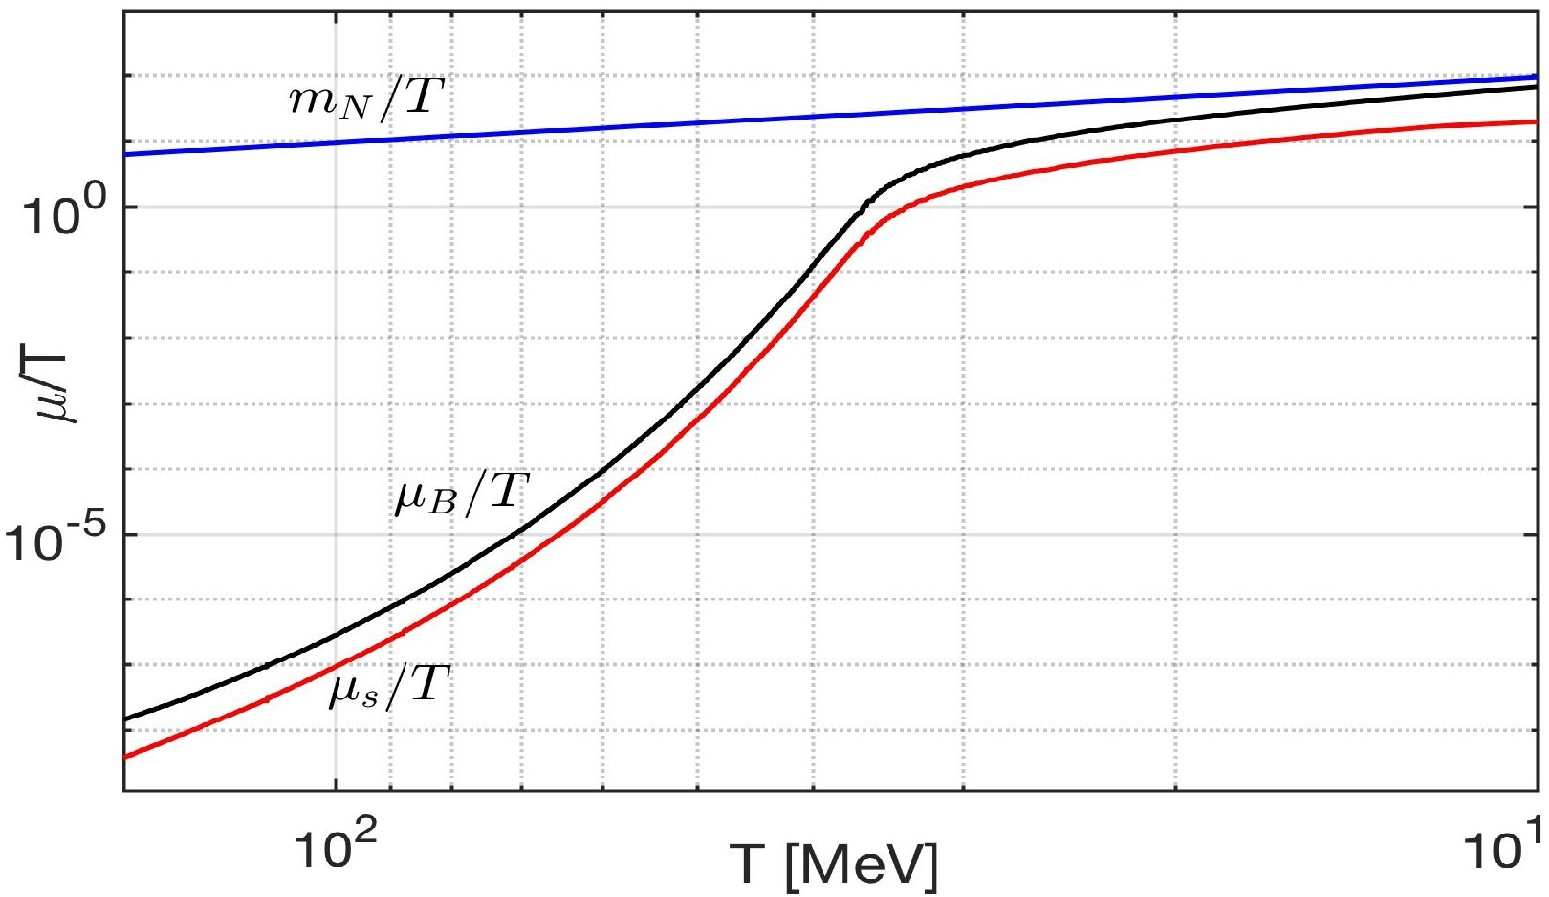
\includegraphics[width=0.9\linewidth]{./plots/New_Chemical_Potential_C.jpg}}
\caption{The chemical potential of baryon number $\mu_B/T$ and strangeness $\mu_s/T$ as a function of temperature $150\MeV> T>10\MeV$ in the primordial Universe; for comparison we show $m_N/T $ with $m_N=938.92\MeV$, the average nucleon mass. \cccite{Yang:2021bko}. \radapt{Yang:2024ret}}
\label{ChemPotFig}\index{chemical potential!baryon}\index{strangeness!chemical potential} 
\end{figure}
%%%%%%%%%%%%%%%%%%%%%%%%%%%%%%

The chemical potential in~\rf{ChemPotFig} changes dramatically in the temperature window $50\MeV\le T\le 30\MeV$, its behavior is describing the antibaryon\index{baryon!antibaryon} disappearance from Universe inventory. Substituting the chemical potential $\lambda_q$ and $\lambda_s$ into particle density \req{Density_N}, \req{Density_K}, and \req{Density_Y}, we can obtain the particle number densities for different species as a function of temperature.

%%%%%%%%%%%%%%%%%%%%%%%%%%%%%%%%%%%%%%%
\begin{figure} 
\centerline{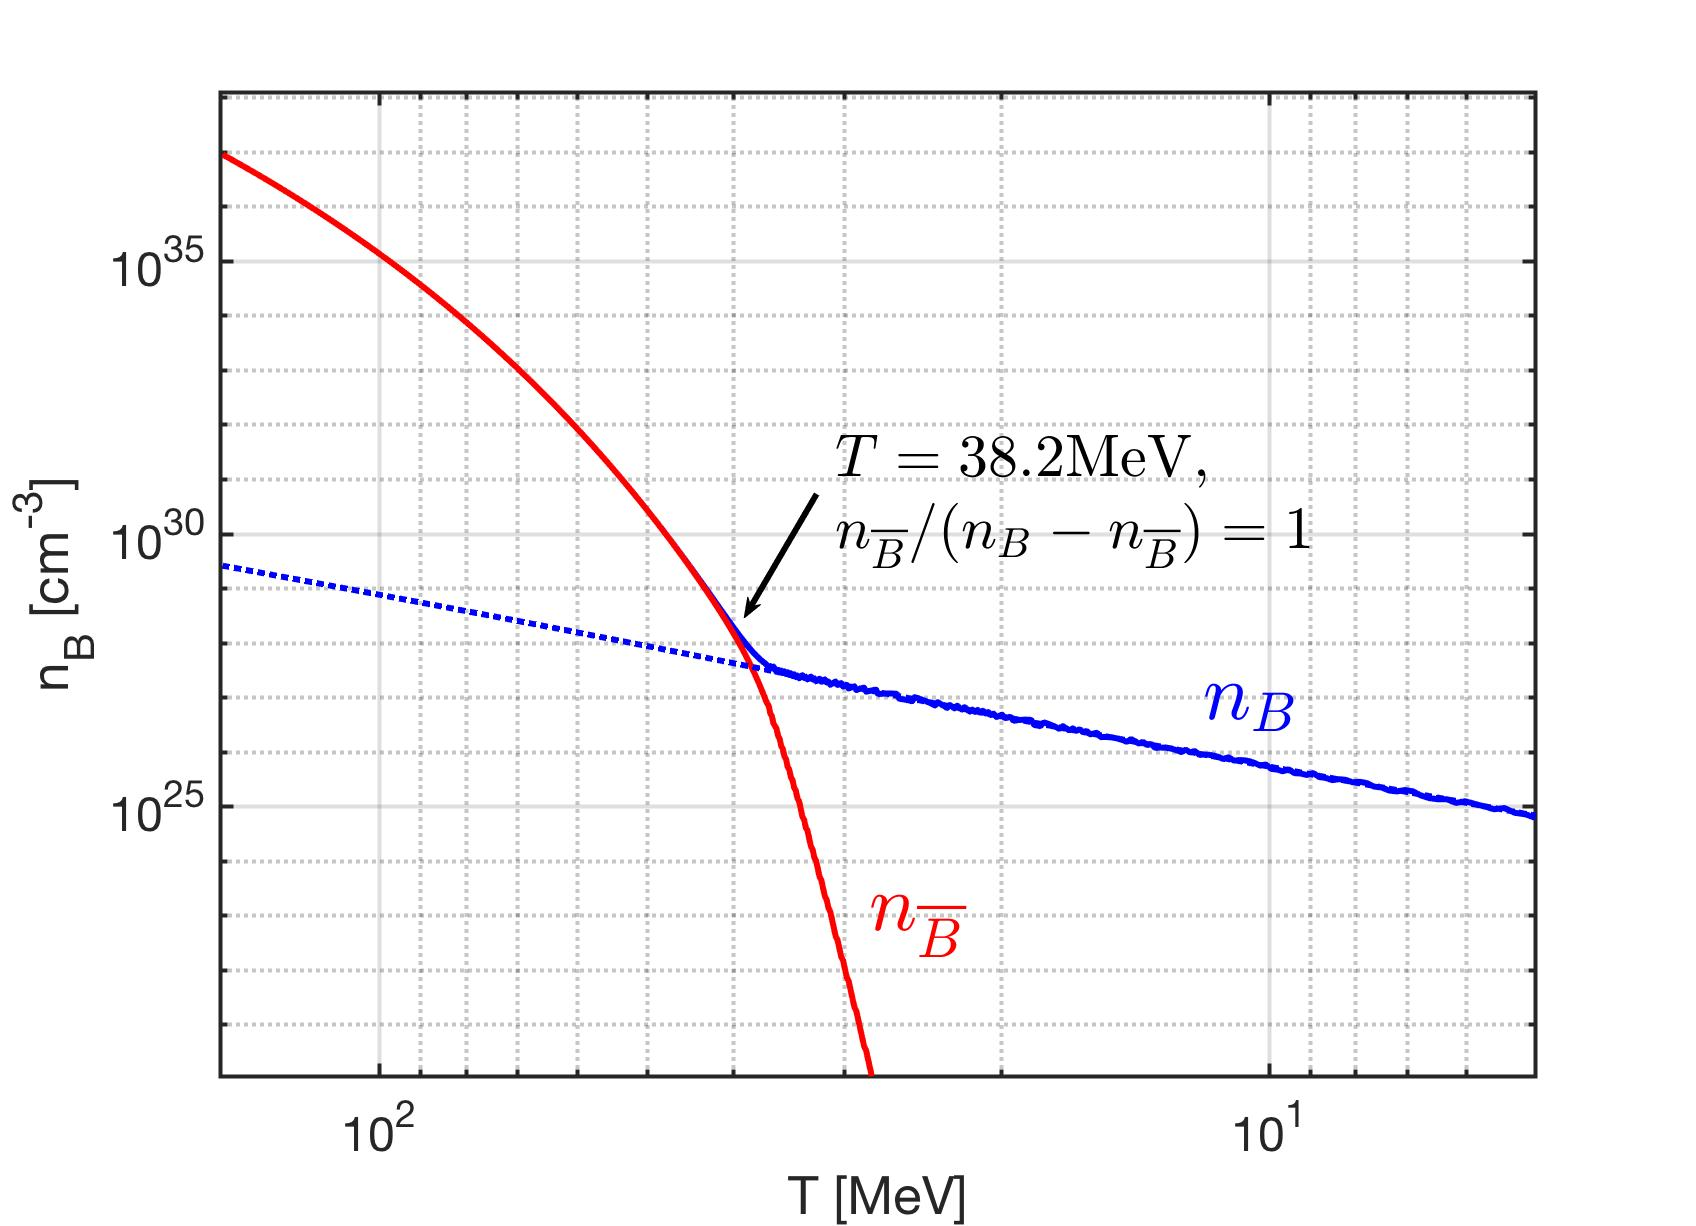
\includegraphics[width=0.9\linewidth]{./plots/Baryon_Antibaryon_cm.jpg}}
\caption{The antibaryon $n_{\overline  B}$ (red solid line) number density as a function of temperature in the range $150\MeV>T>5\MeV$. The blue solid line for baryons  $n_{B}$ merges into the antibaryon yield so that net baryon number $n_{B}-n_{\overline r B}$ (dashed blue line) continues the net  baryon yield seen as solid blue line. At temperature $T=38.2\MeV$  we have $n_{\overline B}/(n_B-n_{\overline B})=1$, antibaryons disappear from the Universe. \cccite{Rafelski:2023emw}. \radapt{Yang:2024ret}}
\label{Baryon:fig}
\end{figure}
%%%%%%%%%%%%%%%%%%%%%%%%%%%%%%%%%%%%%%%

In~\rf{Baryon:fig} we plot the number density of antibaryons (red line),  baryons (solid blue) and net baryon $n_B-n_{\overline B}$ (dashed blue) as a function of temperature. We determine the value of temperature $T=38.2\MeV$ to correspond to the condition $n_{\overline B}\ll(n_B-n_{\overline B})=1$, the effective antibaryon  disappearance temperature from the Universe inventory   $T=38.2\MeV$ is in agreement with the qualitative result presented in 1990 by Kolb and Turner~\cite{Kolb:1990vq}. Below this temperature, there antibaryons rapidly disappear, the net baryon density is the baryon asymmetry which dilutes keeping baryon to entropy ratio constant.

In~\rf{EquilibPartRatiosFig} we show examples of particle abundance ratios of interest\index{hadrons!number ratios}. Pions $\pi(q\bar q)$ are the most abundant hadrons $n_\pi/n_B\gg1$, because of their low mass and the reaction $\gamma\gamma\rightarrow\pi^0$, which assures chemical yield equilibrium~\cite{Kuznetsova:2008jt} in the era of interest here. For $150\MeV>T>20.8\MeV$, we see the ratio $n_{{\overline K}(\bar q s)}/n_B\gg1$, which implies pair abundance of strangeness is more abundant than baryons, and is dominantly present in mesons, since $n_{\overline K}/n_Y\gg1$.  Considering $n_Y/n_B$ we see that hyperons\index{hyperon} $Y(sqq)$ remain a noticeable 1\% component in the baryon yield through the domain of antibaryon decoupling.

%%%%%%%%%%%%%%%%%%%%%%%%%%%%
\begin{figure} 
\centerline{
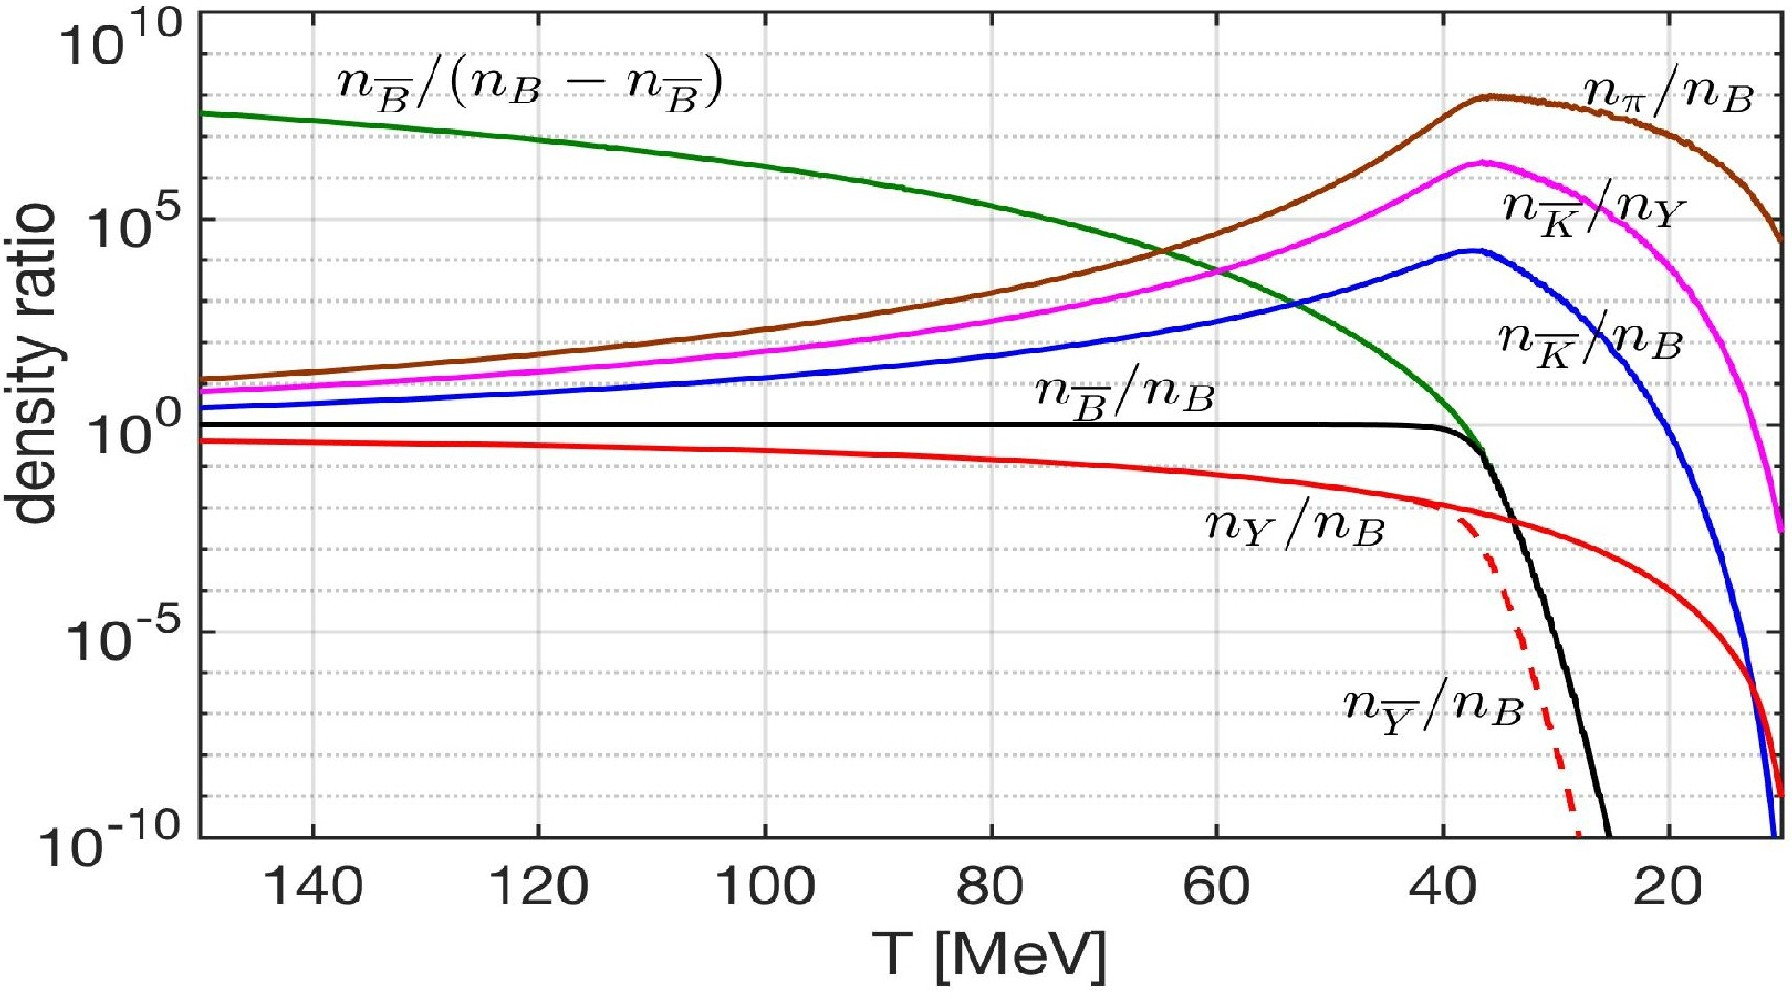
\includegraphics[width=0.9\linewidth]{./plots/Meson_Baryon_density_ratio_C.jpg}}
\caption{Ratios of hadronic particle number densities  with baryon $B$ yields as a function of temperature $150\MeV> T>10\MeV$: Pions $\pi$ (brown line), kaons $K( q\bar s)$ (blue), antibaryon $\overline B$ (black), hyperon $Y$ (red) and anti-hyperons $\overline Y$ (dashed red). Also shown $\overline K/Y$(purple). \cccite{Rafelski:2023emw}. \radapt{Yang:2021bko}}
\label{EquilibPartRatiosFig} 
\end{figure}
%%%%%%%%%%%%%%%%%%%%%%%%%%%
\index{strangeness!equilibrium among baryons and mesons} 

For $20.8\MeV>T$, the  baryon abundance becomes dominant over strange mesons $n_{\overline K}/n_B<1$, which implies that the strange meson is embedded in a large background of baryons, and the exchange reaction $\overline{K}+N\rightarrow \Lambda+\pi$ can re-equilibrate kaons and hyperons in the temperature range; therefore strangeness symmetry $s=\bar s$ can be maintained. For $12.9\MeV>T$ we have $n_Y/n_B>n_{\overline K}/n_B$, now the still existent tiny abundance of strangeness is found predominantly in hyperons.

%%%%%%%%%%%%%%%%%%%%%%%%%%%%%%%%%
\para{Strangeness dynamic population}\index{strangeness!dynamic population}
Given the equilibrium abundances of hadrons in the epoch of interest is $150\MeV\ge T\ge 10\MeV$ we turn now to study the freeze-out temperature for different particles and strangeness  by comparing the relevant reaction rates with each other and with the Hubble expansion rate.  We will need to explore a large number of reactions, going well beyond the relative simplicity of the case of QGP phase of matter. We find that strangeness is kept in equilibrium in the primordial Universe down until $T\approx 13\MeV$. This study addresses non-interacting particles, nuclear interactions can be many times greater compared to this temperature. Thus further exploration of this result seems necessary in the future.

Let us first consider an unstable strange particle $S$ decaying into two particles $1$ and $2$, which themselves have no strangeness content. In a dense and high-temperature plasma with particles $1$ and $2$ in thermal equilibrium, the inverse reaction populates the system with particle $S$. This is written schematically as
\begin{align}
 S\Longleftrightarrow1+2,\qquad \mathrm{Example}: K^0\Longleftrightarrow\pi+\pi\,.
\end{align}
As long as both decay and production reactions are possible, particle $S$ abundance remains in thermal equilibrium; as already discussed this balance between production and decay rates is the `detailed balance'.

Once the primordial Universe expansion rate $1/H$ overwhelms the strongly temperature dependent back-reaction and the back reaction freeze-out, then the decay $S\rightarrow 1+2$ occurs out of balance and particle $S$ disappears rather rapidly from the inventory. 

Second on our list are the two-on-two strangeness producing and burn-up reactions. These have a significantly higher strangeness production reaction threshold, thus especially near to strangeness decoupling their influence is negligible. Such reactions are more important near the QGP hadronization temperature $T_H\simeq 150\MeV$. Typical  strangeness exchange reaction is $\mathrm{K}+N\leftrightarrow \Lambda+\pi$, (see Chapter 18 in~Ref.\,\cite{Letessier:2002ony}).

In~\rf{Strangeness_map2} we show some reactions relevant to strangeness evolution in the considered Universe evolution epoch $150\MeV\ge T\ge 10\MeV$ and their pertinent reaction strength. Specifically:
\begin{itemize}
\item
We study strange quark abundance in baryons and mesons, considering both open and hidden strangeness (hidden: $s\bar s$-content). Important source reactions are $l^-+l^+\rightarrow\phi$, $\rho+\pi\rightarrow\phi$, $\pi+\pi\rightarrow K_\mathrm{S}$, $\Lambda \leftrightarrow \pi+ N$, and $\mu^\pm+\nu\rightarrow K^\pm$. 
\item
Muons\index{muon} and pions are coupled through electromagnetic reactions $\mu^++\mu^-\leftrightarrow\gamma+\gamma$ and $\pi\leftrightarrow\gamma+\gamma$ to the photon background and retain their chemical equilibrium\index{chemical equilibrium} until the temperature $T =4$\, MeV and $T=5\MeV$, respectively~\cite{Rafelski:2021aey,Kuznetsova:2008jt}. The large $\phi\leftrightarrow K+K$ rate assures $\phi$ and $K$ are in relative chemical equilibrium.
\end{itemize}

%%%%%%%%%%%%%%%%%%%%%%%%%%%%%%%%%%%%%%%
\begin{figure} 
\centerline{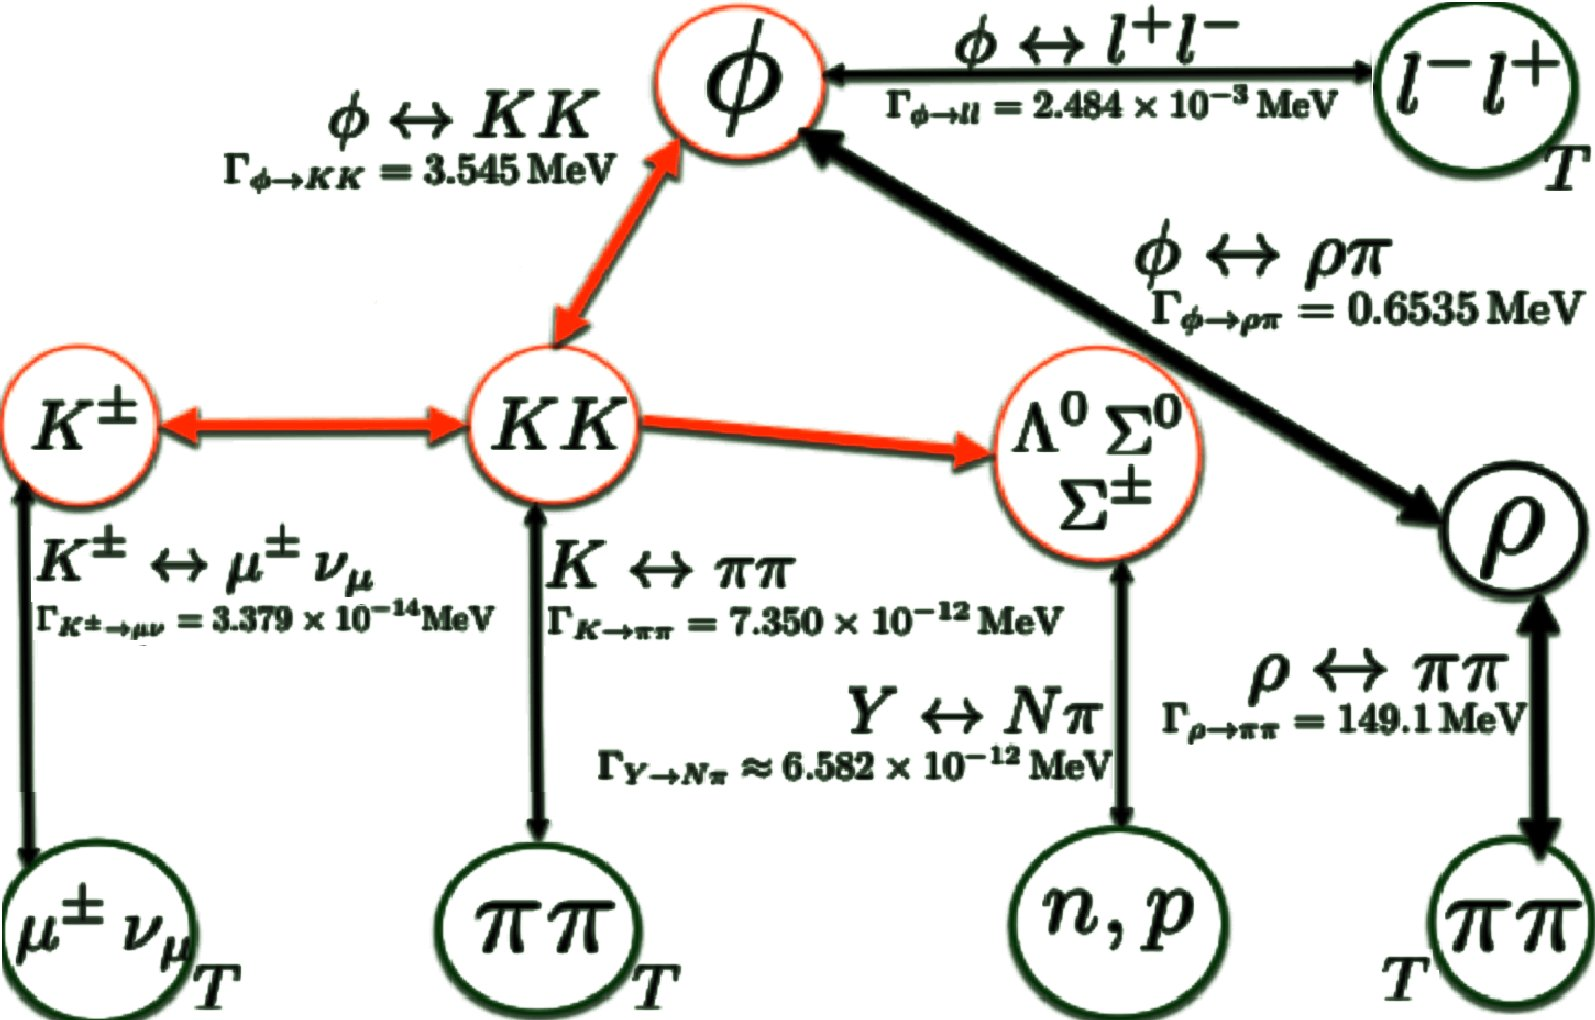
\includegraphics[width=0.9\linewidth]{./plots/Strangeness002_newJ.jpg}}
\caption{The strangeness abundance changing reactions in the primordial Universe. The red circles show strangeness carrying hadronic particles; red thick lines denote effectively instantaneous reactions. Black thick lines show relatively strong hadronic reactions. The reaction rates required to describe strangeness time evolution are presented in Ref.~\cite{Rafelski:2020ajx}. \cccite{Rafelski:2023emw}. \radapt{Yang:2024ret,Yang:2021bko}}
\label{Strangeness_map2} 
\end{figure}
%%%%%%%%%%%%%%%%%%%%%%%%%%%%%%%%%%%%

In order to determine where exactly strangeness disappears from the Universe inventory, we explore the magnitudes of different rates of production and decay processes in mesons and hyperons.
 
%%%%%%%%%%%%%%%%%%%%%%%%%%%%%%%%%%%%%
\para{Strangeness creation and annihilation rates in mesons}
From~\rf{Strangeness_map2} in the meson domain, the relevant interaction rates competing with Hubble time\index{Hubble!time} are the reactions\index{strangeness!mesons production rate}
\begin{align}
 &\pi+\pi\leftrightarrow K\,,\quad\mu^\pm+\nu\leftrightarrow K^\pm\,,\quad l^++l^-\leftrightarrow\phi\,,\\
 &\rho+\pi\leftrightarrow\phi\,,\quad \pi+\pi\leftrightarrow\rho\,.
\end{align}
The thermal reaction rate per time and volume for two body-to-one particle reactions $1+2\rightarrow 3$ has been presented before~\cite{Koch:1986ud,Kuznetsova:2008jt,Kuznetsova:2010pi}. 

In full kinetic and chemical equilibrium, the reaction rate per time per volume can be written as~\cite{Kuznetsova:2010pi} :\index{inverse decay rate}
\begin{align}
&R_{12\to 3}=\frac{g_3}{(2\pi)^2}\,\frac{m_3}{\tau^0_3}\,\int^\infty_0\frac{p^2_3dp_3}{E_3}\frac{e^{E_3/T}}{e^{E_3/T}\pm1}\Phi(p_3)\;,
\end{align}
where $\tau^0_3$ is the vacuum lifetime of particle $3$. The positive sign `$+$' is for the case when particle $3$ is a boson, and negative sign `$-$' for a fermion. The function $\Phi(p_3)$ for the nonrelativistic limit $m_3\gg p_3,T$ can be written as 
\begin{align}
\Phi(p_3\to0)=2\frac{1}{(e^{E_1/T}\pm1)(e^{E_2/T}\pm1)}.
\end{align}

Considering the Boltzmann\index{Boltzmann!approximation} limit, the thermal reaction rate per unit time and volume becomes
\begin{align}
\label{Thermal_Rate}
R_{12\rightarrow3}=\frac{g_3}{2\pi^2}\left(\frac{T^3}{\tau^0_3}\right)\left(\frac{m_3}{T}\right)^2\,K_1(m_3/T),
\end{align}
where $K_1$ is the modified Bessel\index{Bessel function} functions of integer order `$1$'. 

In order to compare the reaction time with Hubble time $1/H$, it is convenient to define the relaxation time for the process $1+2\rightarrow 3$ as follows:
\begin{align}
\label{Reaction_Time}
\tau_{12\rightarrow 3}\equiv\frac{n^{eq}_{1}}{R_{12\rightarrow n}}\,,\quad
n^{eq}_1=\frac{g_1}{2\pi^2}\int_{m_1}^\infty\!\!\!\!dE\,\frac{E\,\sqrt{E^2-m_1^2}}{\exp{\left(E/T\right)}\pm1}\;, 
\end{align}
where $n^{eq}_1$\,is the thermal equilibrium number density of particle\,$1$ with the `heavy' mass $m_1>T$. Combining \req{Thermal_Rate} with \req{Reaction_Time} we obtain
\begin{align}\label{RelaxationTime}
&\frac{\tau_{12\rightarrow3}}{ \tau^0_3}= 
\frac{2\pi^2 n^{eq}_1/T^3}{g_3(m_3/T)^2\,K_1(m_3/T)}\,, \quad 
n^{eq}_1\simeq g_1\left(\frac{m_1 T}{2\pi}\right)^{3/2}e^{-m_1/T}\,,
\end{align}
where, conveniently, the relaxation time does not depend on the abundant and often relativistic heat bath component $2$, \eg\ $l^\pm,\pi,\nu,\gamma$. The density of heavy particles\,$1$\,and\,$3$ can in general be well approximated using the leading and usually nonrelativistic Boltzmann term as shown above.

In general, the reaction rates for inelastic collision process capable of changing particle number, for example $\pi\pi\to K^0$, is suppressed by the factor $\exp{(-m_{K^0}/T)}$. On the other hand, there is no suppression for the elastic momentum and energy exchanging particle collisions in plasma. In general for the case $m\gg T$, the dominant collision term in the relativistic Boltzmann equation is the elastic collision term, keeping all heavy particles in kinetic energy equilibrium with the plasma. This allows us to study the particle abundance in plasma presuming the energy-momentum statistical distribution  equilibrium shape exists.  This insight was discussed in detail in the preparatory phase of laboratory exploration of hot hadron and quark matter, see~\cite{Koch:1986ud}. 

In order to study the particle abundance in the Universe when $m\gg T$, instead of solving the exact Boltzmann equation, we can separate the fast energy-momentum equilibrating collisions from the slow particle number changing inelastic collisions. This approach makes it possible to explore the rates of inelastic collision and compare the relaxation times of particle production in all relevant reactions with the Universe expansion rate at a fixed temperature which governs the shape of particle distributions.

It is common to refer to particle freeze-out as the epoch where a given type of particle ceases to interact with other particles. In this situation the particle abundance decouples from the cosmic plasma, a chemical nonequilibrium and even complete abundance disappearance of this particle can accompany this; the condition for the given reaction $1+2\rightarrow 3$ to decouple is
\begin{align}
\tau_{12\rightarrow 3}(T_f)=1/H(T_f),
\end{align}
where $T_f$ is the freeze-out temperature.

In the epoch of interest, $150\MeV>T>10\MeV$, the Universe is dominated by radiation and effectively massless matter behaving like radiation. The Hubble parameter can be obtained from the Hubble equation and written as~\cite{Kolb:1990vq}
\begin{align}\label{H2g}
H^2=H^2_{rad}\left(1+\frac{\rho_{\pi,\,\mu,\,\rho}}{\rho_\mathrm{rad}}+\frac{\rho_\mathrm{strange}}{\rho_\mathrm{rad}}\right)=\frac{8\pi^3G_\mathrm{N}}{90}g^e_\ast T^4,\qquad H^2_\mathrm{rad}=\frac{8\pi G_\mathrm{N}\,\rho_\mathrm{rad}}{3},
\end{align}
where: $g^e_\ast$ is the total number of effective relativistic `energy' degrees of freedom; $G_\mathrm{N}$ is the Newtonian constant of gravitation; the `radiation' energy density includes $\rho_\mathrm{rad}=\rho_\gamma+\rho_\nu+\rho_{e^\pm}$ for photons, neutrinos, and massless electrons(positrons). The massive-particle correction is $\rho_{\pi,\,\mu,\,\rho}=\rho_\pi+\rho_\mu+\rho_\rho$; and at highest $T$ of interest, also of (minor) relevance, $\rho_\mathrm{strange}=\rho_{K^0}+\rho_{K^\pm}+\rho_{K^\ast}+\rho_{\eta}+\rho_{\eta^\prime}$.
Equating $1/H$ to the computed reaction rate we obtain the freeze-out temperature $T_f$. 

When considering the reaction rates and quoting $T_f$,   we must check allowing for a finite reaction time how sudden the freeze-out happens. We refer to this temperature uncertainty as  $\Delta T_f$, which by a simple scale consideration can be defined by
\begin{equation}\label{eq:DeltaT}
\Delta T_f\simeq \frac{1}{R(T_f)}\times \frac{dT}{dt}\,. 
\end{equation}
$R$\,[MeV] is the value of reaction rate at freeze-out. The greater is the rate $R_f$ the sharper is the freeze-out, thus smaller $\Delta T_f$.\index{freeze-out!uncertainty}

For the temperature range $50\MeV>T>5\MeV$, we have $10^{-1}<dT/dt<10^{-4}\MeV$/$\mu$s. We estimate the  width of freeze-out temperature interval $\Delta T_f$ using reaction rates for $dt$ as follows
\begin{align}
\frac{1}{\Delta T_f}\equiv \left[\frac{1}{(\Gamma_{12\to3}/H)}\frac{d(\Gamma_{12\to3}/H)}{dT}\right]_{T_f},\quad \Gamma_{12\to3}\equiv\frac{1}{\tau_{12\to3}}.
\end{align}
Using \req{H2g} and \req{RelaxationTime} and considering the temperature range $50\MeV>T>5\MeV$ with $g^e_\ast\approx\mathrm{constant}$ we obtain using the Boltzmann approximation to describe the massive particles\,$1$\,and\,$3$
\begin{align}\label{DeltaFreezeout}
 \frac{\Delta T_f}{ T_f} \approx\frac{T_f }{ m_3 - m_1 -2T_f}\,,\quad m_3 - m_1>> T_f\,.
\end{align}
The width of freeze-out domain is shown in the right column in Table~\ref{FreezeoutTemperature_table}. We see a range of $2$-$10\%$. Therefore it is nearly justified to consider as a decoupling condition in time the value of temperature at which the pertinent rate crosses the Hubble expansion rate, see~\rf{reaction_time_tot}.\index{freeze-out!duration}
 
%%%%%%%%%%%%%%%%%%%%%%%%%%%
\begin{table} 
\centering
\begin{tabular}{c| c| c}
\hline\hline
Reactions &Freeze-out $T_f$\,[MeV] & {Uncertainty $\Delta T_f$\,[MeV]} \\
\hline
$\mu^\pm\nu\rightarrow K^\pm$ & $T_f=33.8\MeV$ & {$3.5$ \,MeV}\\ 
\hline
$e^+e^-\rightarrow \phi$ & $T_f=24.9\MeV$ &{$0.6\MeV$}\\
$\mu^+\mu^-\rightarrow\phi$ & $T_f=23.5\MeV$ &{$0.6\MeV$}\\
\hline
 $\pi\pi\rightarrow K$ & $T_f=19.8\MeV$&{$1.2\MeV$}\\
\hline
$\pi\pi\rightarrow\rho$ & $T_f=12.3\MeV$&{$0.2\MeV$}\\
\hline\hline
\end{tabular}
\caption{Strangeness producing reactions in primordial Universe, their freeze-out temperature $T_f$; and temperature uncertainty $\Delta T_f$}
\label{FreezeoutTemperature_table} 
\end{table}
%%%%%%%%%%%%%%%%%%%%%%%%%%%%%%%%%%%%%%

%%%%%%%%%%%%%%%%%%%%%%%%%%%%%%%%%%%%%%%%%
\begin{figure}
%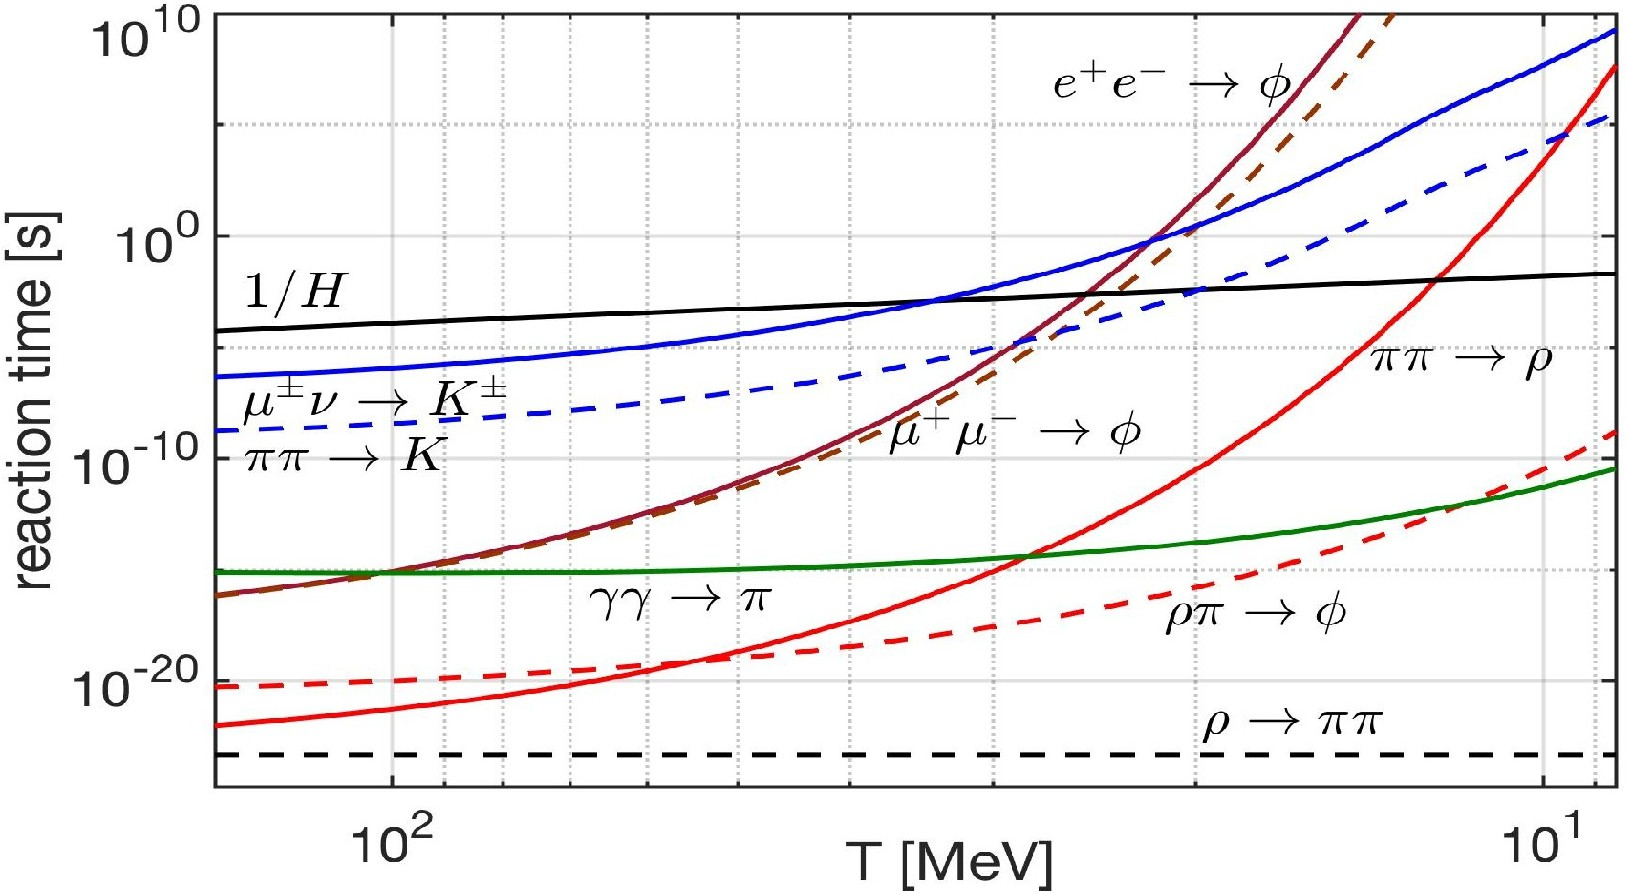
\includegraphics[width=0.95\linewidth]{./plots/Strangeness_Hubble_C.jpg}
\centerline{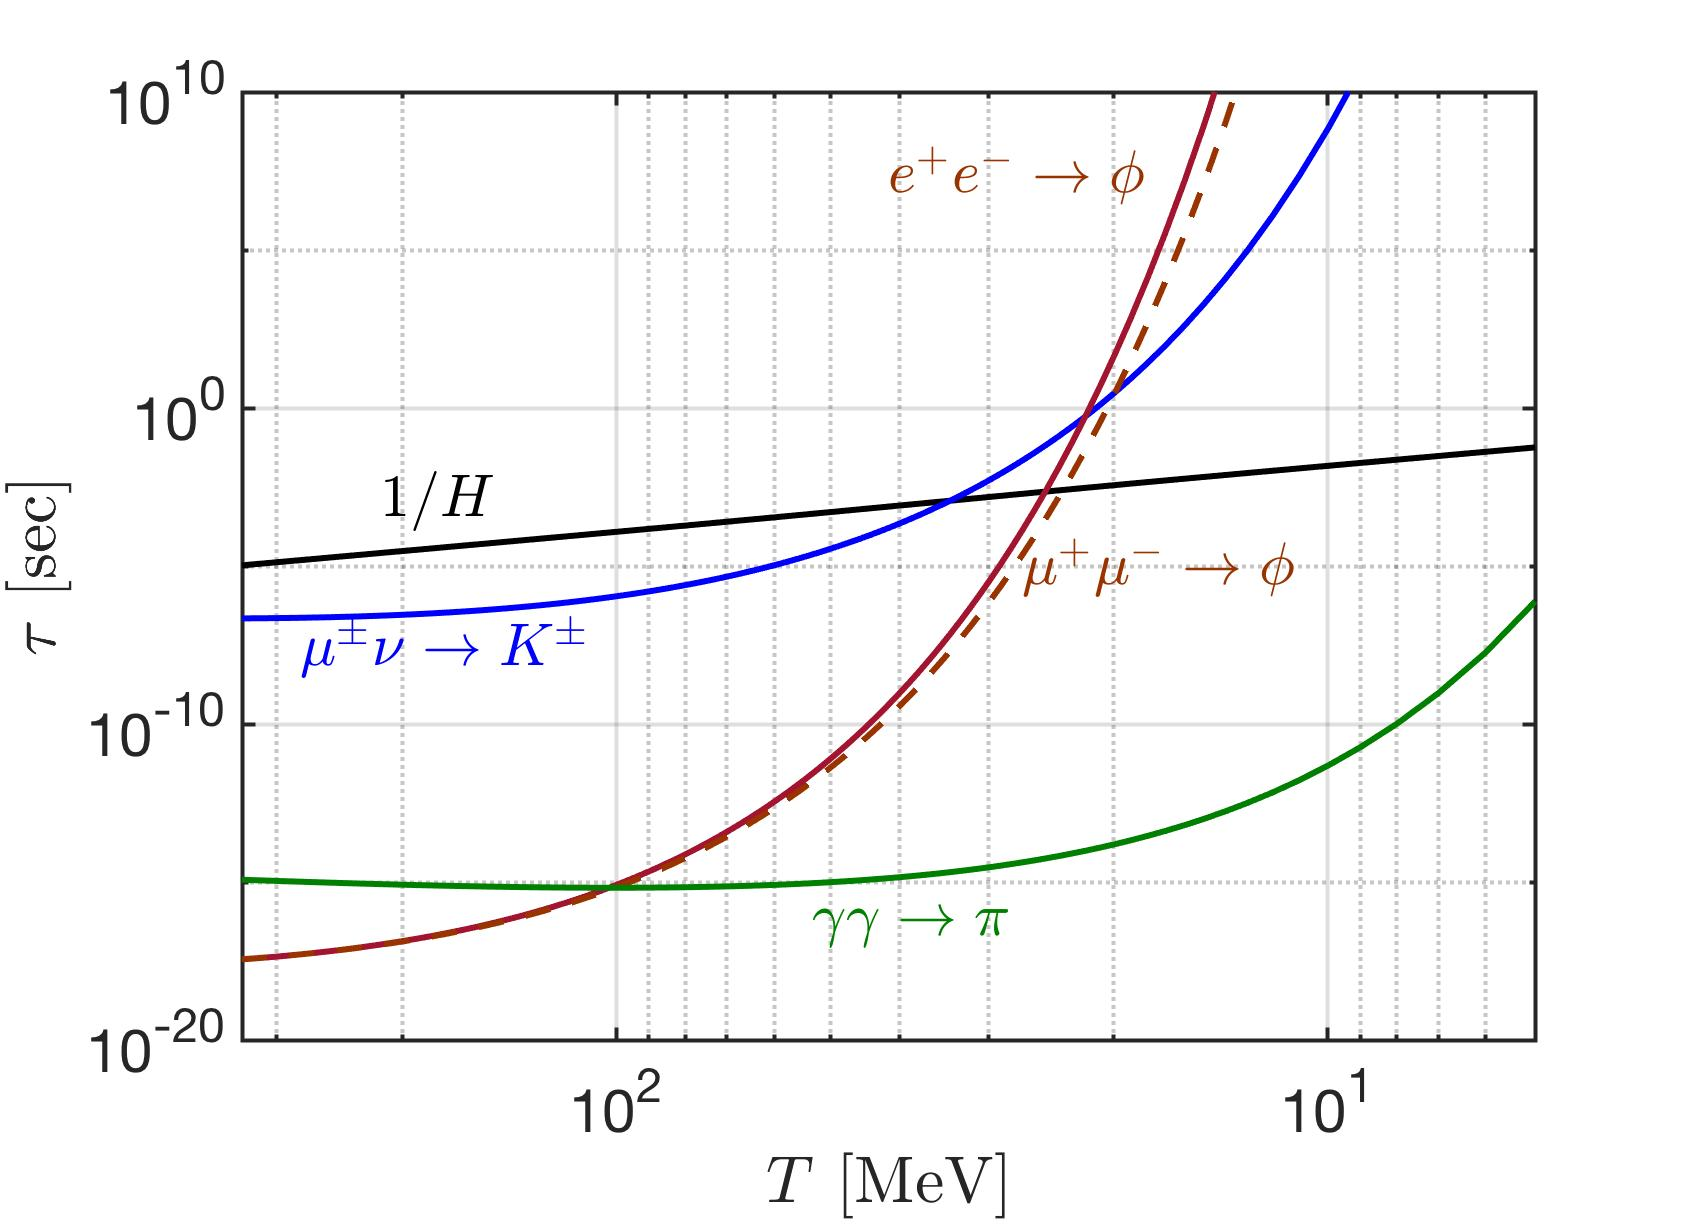
\includegraphics[width=0.9\linewidth]{./plots/Strangeness_Hubble002.jpg}}
\centerline{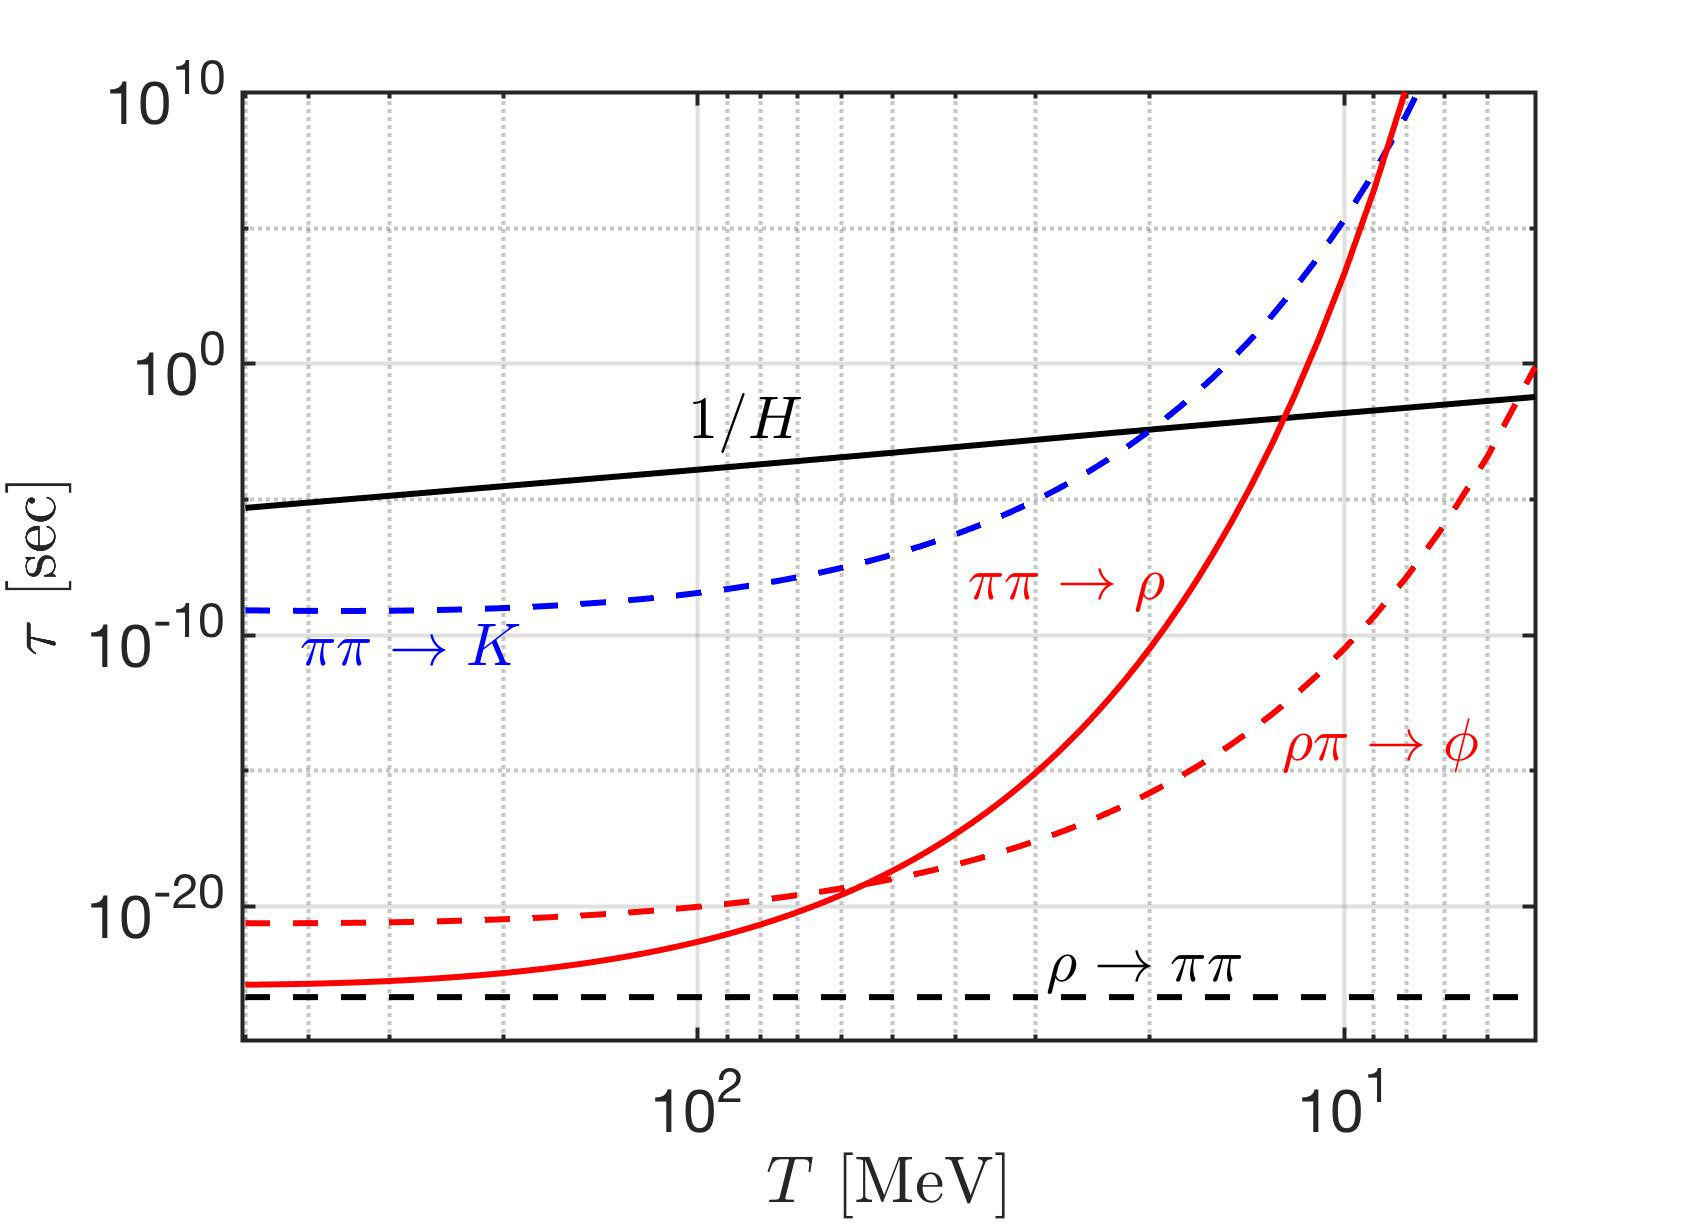
\includegraphics[width=0.9\linewidth]{./plots/Strangeness_Hubble003.jpg}}
\caption{Hadronic relaxation reaction times, see \req{Reaction_Time}, as a function of temperature $T$, are compared to Hubble time $1/H$ (black solid line). At bottom the horizontal black-dashed line is the natural (vacuum) lifespan of $\rho$. \cccite{Rafelski:2023emw}. \radapt{Yang:2024ret,Yang:2021bko}}
\label{reaction_time_tot} 
\end{figure}
%%%%%%%%%%%%%%%%%%%%%%%%

In~\rf{reaction_time_tot} we plot the hadronic reaction relaxation times $\tau_{i}$ in the meson sector as a function of temperature compared to Hubble time $1/H$. We note that the weak interaction reaction $\mu^\pm+\nu_{\mu}\rightarrow K^\pm$ becomes slower compared to the Universe expansion near temperature $T_f^{K^\pm}=33.8\MeV$, signaling the onset of abundance nonequilibrium for $K^\pm$. For $T<T_f^{K^\pm}$, the reactions $\mu^\pm+\nu_{\mu}\rightarrow K^\pm$ decouples from the cosmic plasma; the corresponding detailed balance\index{detailed balance} can be broken and the decay reactions $K^\pm\rightarrow\mu^\pm+\nu_{\mu}$ are acting like a (small) ``hole'' in the strangeness abundance ``pot''. If other strangeness production reactions did not exist, strangeness would disappear as the Universe cools below $T_f^{K^\pm}$. However, there are other reactions: $l^++l^-\leftrightarrow\phi$, $\pi+\pi\leftrightarrow K$, and $\rho+\pi\leftrightarrow\phi$ can still produce the strangeness in cosmic plasma and the rate is very large compared to the weak interaction decay.

In Table~\ref{FreezeoutTemperature_table} we also show the characteristic strangeness reactions and their freeze-out temperatures in the primordial Universe. The intersection of strangeness reaction times with $1/H$ occurs for $l^-+l^+\rightarrow\phi$ at $T_f^\phi=25\sim23\MeV$, and for $\pi+\pi\rightarrow K$ at $T_f^K=19.8\MeV$, for $\pi+\pi\rightarrow\rho$ at $T_f^\rho=12.3\MeV$. The reactions $\gamma+\gamma\rightarrow\pi$ and $\rho+\pi\leftrightarrow\phi$ are faster compared to $1/H$. However, the $\rho\to\pi+\pi$ lifetime (black dashed line in~\rf{reaction_time_tot}) is smaller than the reaction $\rho+\pi\leftrightarrow\phi$; in this case, most of $\rho$-meson decays faster, thus are absent and cannot contribute to the strangeness creation in the meson sector. Below the temperature $T<20\MeV$, all the detail balances in the strange meson reactions are broken and the strangeness in the meson sector should disappear rapidly, were it not for the small number of baryons present in the Universe.

%%%%%%%%%%%%%%%%%%%%%%%%%%%%%%%%%%%%%%%%%%%%
\para{Strangeness production and exchange rates involving hyperons}\index{strangeness!hyperons}
In order to understand strangeness in hyperons in the baryonic domain, we now consider the strangeness production reaction $\pi +N\rightarrow K+\Lambda$, the strangeness exchange reaction $\overline{K}+N\rightarrow \Lambda+\pi$; and the strangeness decay $\Lambda\rightarrow N+\pi$. The competition between different strangeness reactions allows strange hyperons and anti-hyperons to influence the dynamic nonequilibrium condition, including development of $\langle s-\bar s\rangle \ne 0$.

To evaluate the reaction rate in two-body reaction $1+2\rightarrow3+4$ in the Boltzmann approximation\index{Boltzmann!approximation} we can use the reaction cross section $\sigma(s)$ and the relation~\cite{Letessier:2002ony}:\index{hyperon!production rate}
\begin{align}
R_{12\rightarrow34}=\frac{g_1g_2}{32\pi^4}\frac{T}{1+I_{12}}\!\!\int^\infty_{s_{th}}\!\!\!\!ds\,\sigma(s)\frac{\lambda_2(s)}{\sqrt{s}}\!K_1\!\!\left({\sqrt{s}}/{T}\right),
\end{align}
where $K_1$ is the Bessel\index{Bessel function} function of order $1$ and the function $\lambda_2(s)$ is defined as
\begin{align}
\lambda_2(s)=\left[s-(m_1+m_2)^2\right]\left[s-(m_1-m_2)^2\right],
\end{align}
with $m_1$ and $m_2$, $g_1$ and $g_2$ as the masses and degeneracy of the initial interacting particle. The factor $1/(1+I_{12})$ is introduced to avoid double counting of indistinguishable pairs of particles; we have $I_{12}=1$ for identical particles and $I_{12}=0$ for others. 

The thermal averaged cross sections for the strangeness production and exchange processes are about $\sigma_{\pi N\rightarrow K\Lambda}\sim0.1\,\mathrm{mb}$ and $\sigma_{\overline{K}N\rightarrow \Lambda\pi}=1\sim3\,\mathrm{mb}$ in the energy range in which we are interested~\cite{Koch:1986ud}. The cross section can be parameterized as follows:\\
1) For the cross section $\sigma_{\overline{K}N\rightarrow \Lambda\pi}$ we use~\cite{Koch:1986ud}
 \begin{align}
 \sigma_{\overline{K}N\rightarrow \Lambda\pi}=\frac{1}{2}\left(\sigma_{K^-p\rightarrow \Lambda\pi^0}+\sigma_{K^-n\rightarrow \Lambda\pi^-}\right)\,.
\end{align}
Here the experimental cross sections can be parameterized as 
\begin{align}
&\sigma_{K^-p\rightarrow \Lambda\pi^0}\!\!=\!\!\left(\begin{array}{l}\!\!1479.53\mathrm{mb}\!\cdot\!\exp{\left(\frac{-3.377\sqrt{s}}{\mathrm{GeV}}\right)},\; \mathrm{for}\,\sqrt{s_m}\!\!<\!\!\sqrt{s}\!<\!3.2\mathrm{GeV} \\ \\0.3\mathrm{mb}\!\cdot\!\exp{\left(\frac{-0.72\sqrt{s}}{\mathrm{GeV}}\right)},\; \mathrm{for}\sqrt{s}>3.2\mathrm{GeV}\end{array}\right.\\
&\sigma_{K^-n\rightarrow \Lambda\pi^-}\!\!=\!\!1132.27\mathrm{mb}\!\cdot\!\exp{\left(\frac{-3.063\sqrt{s}}{\mathrm{GeV}}\right)},\; \mathrm{for}\sqrt{s}>1.699\mathrm{GeV},
\end{align}
where $\sqrt{s_m}=1.473\GeV$.\\
2) For the cross section $\sigma_{\pi N\rightarrow K\Lambda}$ we use~\cite{Cugnon:1984pm}
\begin{align}
&\sigma_{\pi N\rightarrow K\Lambda}=\frac{1}{4}\times\sigma_{\pi p\rightarrow K^0\Lambda}\,.
\end{align}
The experimental $\sigma_{\pi p\rightarrow K^0\Lambda}$ can be approximated as follows
\begin{align}
\sigma_{\pi p\rightarrow K^0\Lambda}=\left(\begin{array}{l}\frac{0.9\mathrm{mb}\cdot\left(\sqrt{s}-\sqrt{s_0}\right)}{0.091\mathrm{GeV}},\; \mathrm{for} \sqrt{s_0}<\sqrt{s}<1.7\mathrm{GeV} \\ \\ \frac{90\mathrm{MeV\cdot mb}}{\sqrt{s}-1.6\mathrm{GeV}},\; \mathrm{for}\sqrt{s}>1.7\mathrm{GeV},\end{array}\right.
 \end{align}
 with $ \sqrt{s_0}=m_\Lambda+m_K$. 

Given the cross sections, we obtain the thermal reaction rate per volume for strangeness exchange reaction seen in~\rf{Lambda_Rate_volume.fig}. We see that near to $T=20\MeV$, the dominant reactions for the hyperon\index{hyperon} $\Lambda$ production is $\overline{K}+N\leftrightarrow\Lambda+\pi$. At the same time, the $\pi+\pi\to K$ reaction becomes slower than Hubble time and kaon $K$ decay rapidly in the primordial Universe. However, the anti-kaons $\overline K$ produce the hyperon $\Lambda$ because of the strangeness exchange reaction $\overline{K}+N\rightarrow\Lambda+\pi$ in the baryon-dominated Universe. We have strangeness in $\Lambda$ and it disappears from the Universe via the decay $\Lambda\rightarrow N+\pi$. Both strangeness and anti-strangeness disappear because of the $K\rightarrow\pi+\pi$ and $\Lambda\rightarrow N+\pi$, while the strangeness abundance $s = \bar{s}$ in the primordial Universe remains.

%%%%%%%%%%%%%%%%%%%%%%%%%%%%%%%%
\begin{figure} 
\centerline{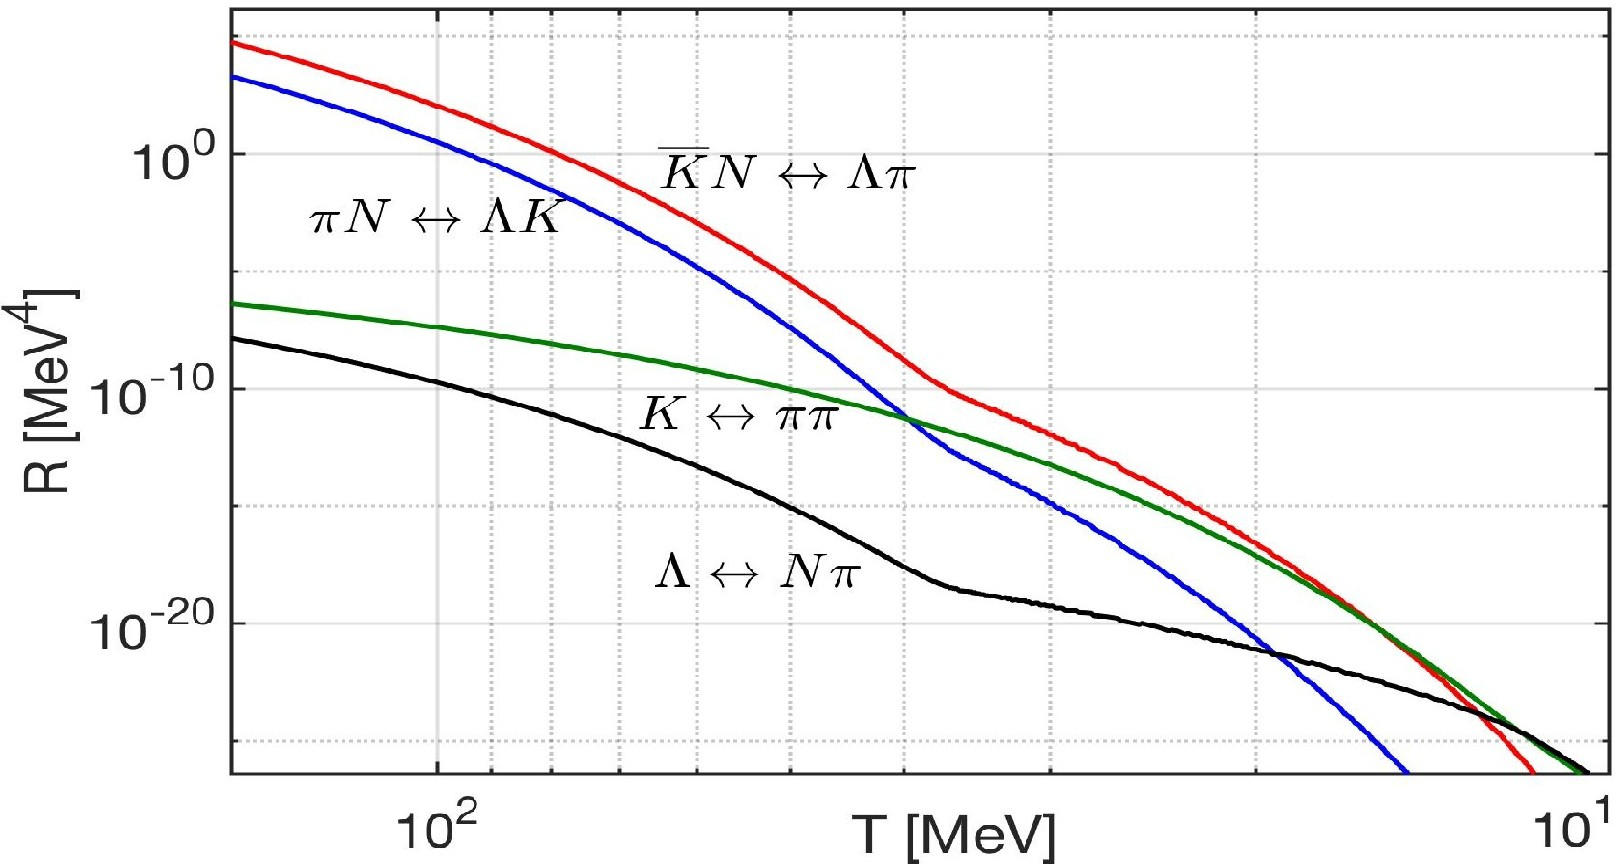
\includegraphics[width=0.9\linewidth]{./plots/NewHyperonRate_C.jpg}}
\caption{Thermal reaction rate $R$ per volume and time for important hadronic strangeness production and exchange processes as a function of temperature $150\MeV> T>10\MeV$ in the primordial Universe. \cccite{Rafelski:2023emw}. \radapt{Yang:2024ret,Yang:2021bko}}
\label{Lambda_Rate_volume.fig} 
\end{figure}
%%%%%%%%%%%%%%%%%%%%%%%%%%%%%%%%%%%%

Near to $T=12.9\MeV$ the reaction $\Lambda+\pi\rightarrow\overline{K}+N$ becomes slower than the strangeness decay $\Lambda\leftrightarrow N+\pi$ and shows that at the low temperature the $\Lambda$ particles are still in equilibrium via the reaction $\Lambda\leftrightarrow N+\pi$ and little strangeness remains in the $\Lambda$. Then strangeness abundance becomes asymmetric $s\gg \bar{s}$, which implies that the assumption for strangeness conservation can only be valid until the temperature $T\sim13\MeV$. Below this temperature a new regime opens up in which the tiny residual strangeness abundance is governed by weak decays with no re-equilibration with mesons. Also, in view of baron asymmetry, $\langle s-\bar s\rangle \ne 0$.
